\documentclass[11pt]{article}
\usepackage[a4paper, margin=1in]{geometry}

\usepackage[hidelinks]{hyperref}
\hypersetup{
	colorlinks=true,
	linkcolor=blue,
}
\usepackage{amsfonts, amsmath, amssymb, amsthm}
\usepackage{graphicx}
\usepackage{subfigure}
\usepackage{caption}
\usepackage{subcaption}
\usepackage{fancyhdr}



\begin{document}
	\begin{titlepage}
		\begin{center}
			\begin{figure}
				\centering
				
\includegraphics[scale=0.15]{images/IUST_Logo.jpg} \\
				\caption*{\textbf{School of Mathematics \& Computer Science}}
			\end{figure}
			\vspace*{0.5cm}
			\Huge{\textbf{Comparison of \\ Numerical Methods and PINNs \\ for the Schrödinger equation}}\\
			\vspace*{3cm}
			\large{\textbf{Mohsen Peykanro}}\\
			\large{\textbf{Ehsan Pichka}}\\
			\large{\textbf{Arshia Soleymani}}\\
			\vspace*{3cm}
			\large{\textbf{Advisor:}}\\
			\large{\textbf{Dr. Mahboubeh Molavi Arabshahi}}\\
			\vspace*{3cm}
			\today
		\end{center}
	\end{titlepage}
	
\section{Introduction}
\subsection{Background}
The Schrödinger equation is a partial differential equation in quantum mechanics that describes how the quantum state of a physical system change over time. This equation can handle the behavior of particles at the microscopic level. This equation have two forms that are based on times. The time-dependent Schrödinger equation describes the change of a system's wave function over time, while the time-independent version is used to determine stationary states and energy levels.

In most cases, you cant solve the equation so the exact analytical solutions are not available, especially for complex potentials or higher-dimensional systems. As a result, numerical methods play a crucial role in approximating solutions. The solution to the Schrödinger equation is called the wave function that provides information about the probability distribution of a particle's position and momentum. We mostly are going to survey Classical numerical approaches and Physics-Informed Neural Networks (PINNs) in this article.

The Classical numerical approaches such as the finite difference method (FDM) and finite element method (FEM) have been widely used for solving partial differential equations like Schrödinger equation. These methods rely on discretization of the domain and typically require careful handling of stability, convergence, and computational cost. On the other hand in recent years, PINNs have appeard as a modern approach for solving differential equations. PINNs merge the physical laws directly into the loss function of a neural network, so the solution will be approximated without discretization of the domain. This makes PINNs usefull for complex and high-dimensional problems.

\subsection{Objective of the Study}
The main objective of this paper is to compare classical numerical methods and Physics-Informed Neural Networks in solving the Schrödinger equation. Despite the growing interest in PINNs, we are not quite sure that how they compare to classical numerical methods in terms of accuracy, efficiency, and stability. A systematic comparison is necessary to evaluate their strengths and limitations.

\section{Mathematical Formulation}
\subsection{Early-Stage Quantum Theory}
The Schrödinger equation is a direct consequence of the discovery of quanta in the early 20th century. Its origins lie in the energy quanta hypothesis proposed by Max Planck in 1900 and the photon hypothesis by Albert Einstein in 1905, which established that energy and momentum are quantized.
\begin{equation}  \label{eq:1905}
	E = h \nu = \hbar \omega
\end{equation} 
where $E$ denotes energy, $h$ is the Plnack constant ($6.626 \times 10^{-34} \,\text{J·s}$) and $\nu$ is frequency of light. so now we can define the reduced Planck constant as $\hbar = \frac{h}{2 \pi}$ and $\omega = 2 \pi \nu$ as angular frequency. 
Later on, Einstein in 1917 concluded that momentum of light quantum $p$ is:
\begin{equation}  \label{eq:1917}
	 p = \frac{E}{c} = \frac{\hbar \omega}{c} = \hbar k 
\end{equation}
$k$ is called wavenumber and is defind as $ k = 2 \pi \lambda$, where $\lambda$ is wavelength of light in vacuum.

In 1923, Arthur Compton conducted experiments investigating how incident X-ray beams were scattered by matter, such as graphite and copper. He discovered a systematic redshift (an increase in wavelength) in the scattered X-rays and they call it Compton effect. Moreover he found that the shift in wavelengths depended only on the scattering angle regardless of quality of material of a scatterer. 
\begin{equation}
	\Delta \lambda = \frac{h}{m_e c} (1 - \cos \theta) 
\end{equation} 
where $\Delta \lambda$ means a Shift in wave length of scatterd beam, $m_e$ is a rest mass of an electron (mass that is independent of the motion of the particle) and $\theta$ is a scatering angle of the beam. The constant $\frac{h}{m_e c} $ is defined as the electron Compton wavelength ( $\lambda_e$) approximately $ 2.426 \times 10^{-12} $ meters.

\begin{figure}[h!]
	\centering
	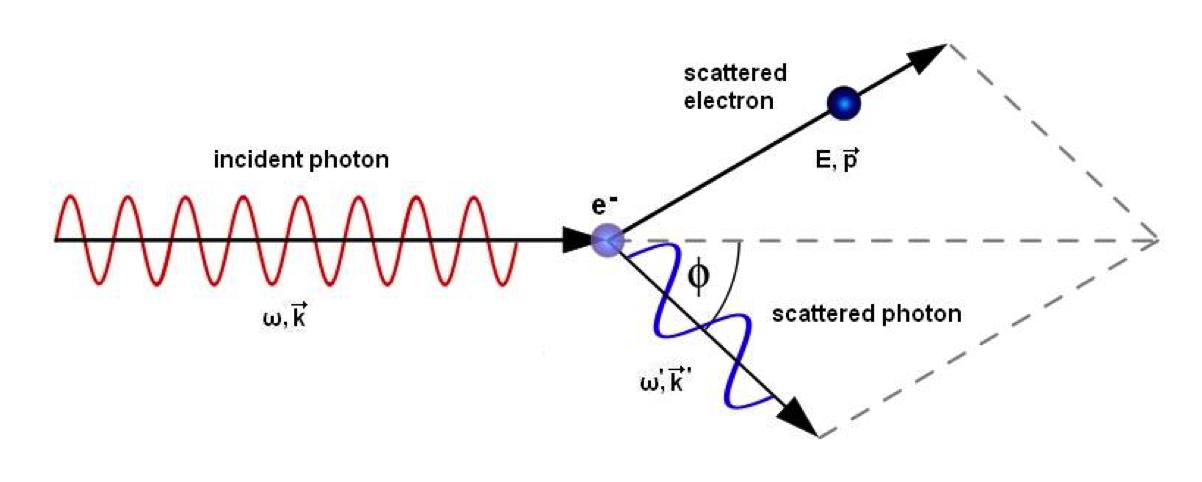
\includegraphics[height=5cm]{images/Fig5}
	\caption{Compton effect: scattering of a photon on a resting electron}
\end{figure}


In 1924, Louis de Broglie Encouraged by the success of Einstein and Compton in proving that waves (light) could behave like particles and theorized that the reverse must also be true, in other word matter particles must possess a wave nature. De Broglie essentially reversed the relationship of (\ref{eq:1905}) and (\ref{eq:1917}) such that
\begin{equation}
	\omega = \frac{E}{\hbar}, \quad k = \frac{p}{\hbar} \quad \text{or} \quad \lambda = \frac{h}{p}
\end{equation}
where $p$ equals $|p|$ and $\lambda$ is a wavelength of a corpuscular beam(a directional stream of tiny particles). this is called de Broglie wavelength (matter wave). this equation implies that if we are able to determine the wavelength of the corpuscular beam experimentally, we can decide a magnitude of momentum accordingly.

For a matter wave, the phase velocity $v_p$ is shown to be greater than $c$, while the group velocity $v_g$, which represents the propagation velocity of a wave packet (and thus the particle's velocity), is less than $c$. Their relationship is defined by $v_p v_g = c^2$. Therefore, a particle velocity must not exceed $c$.
\begin{figure}[h!]
	\centering
	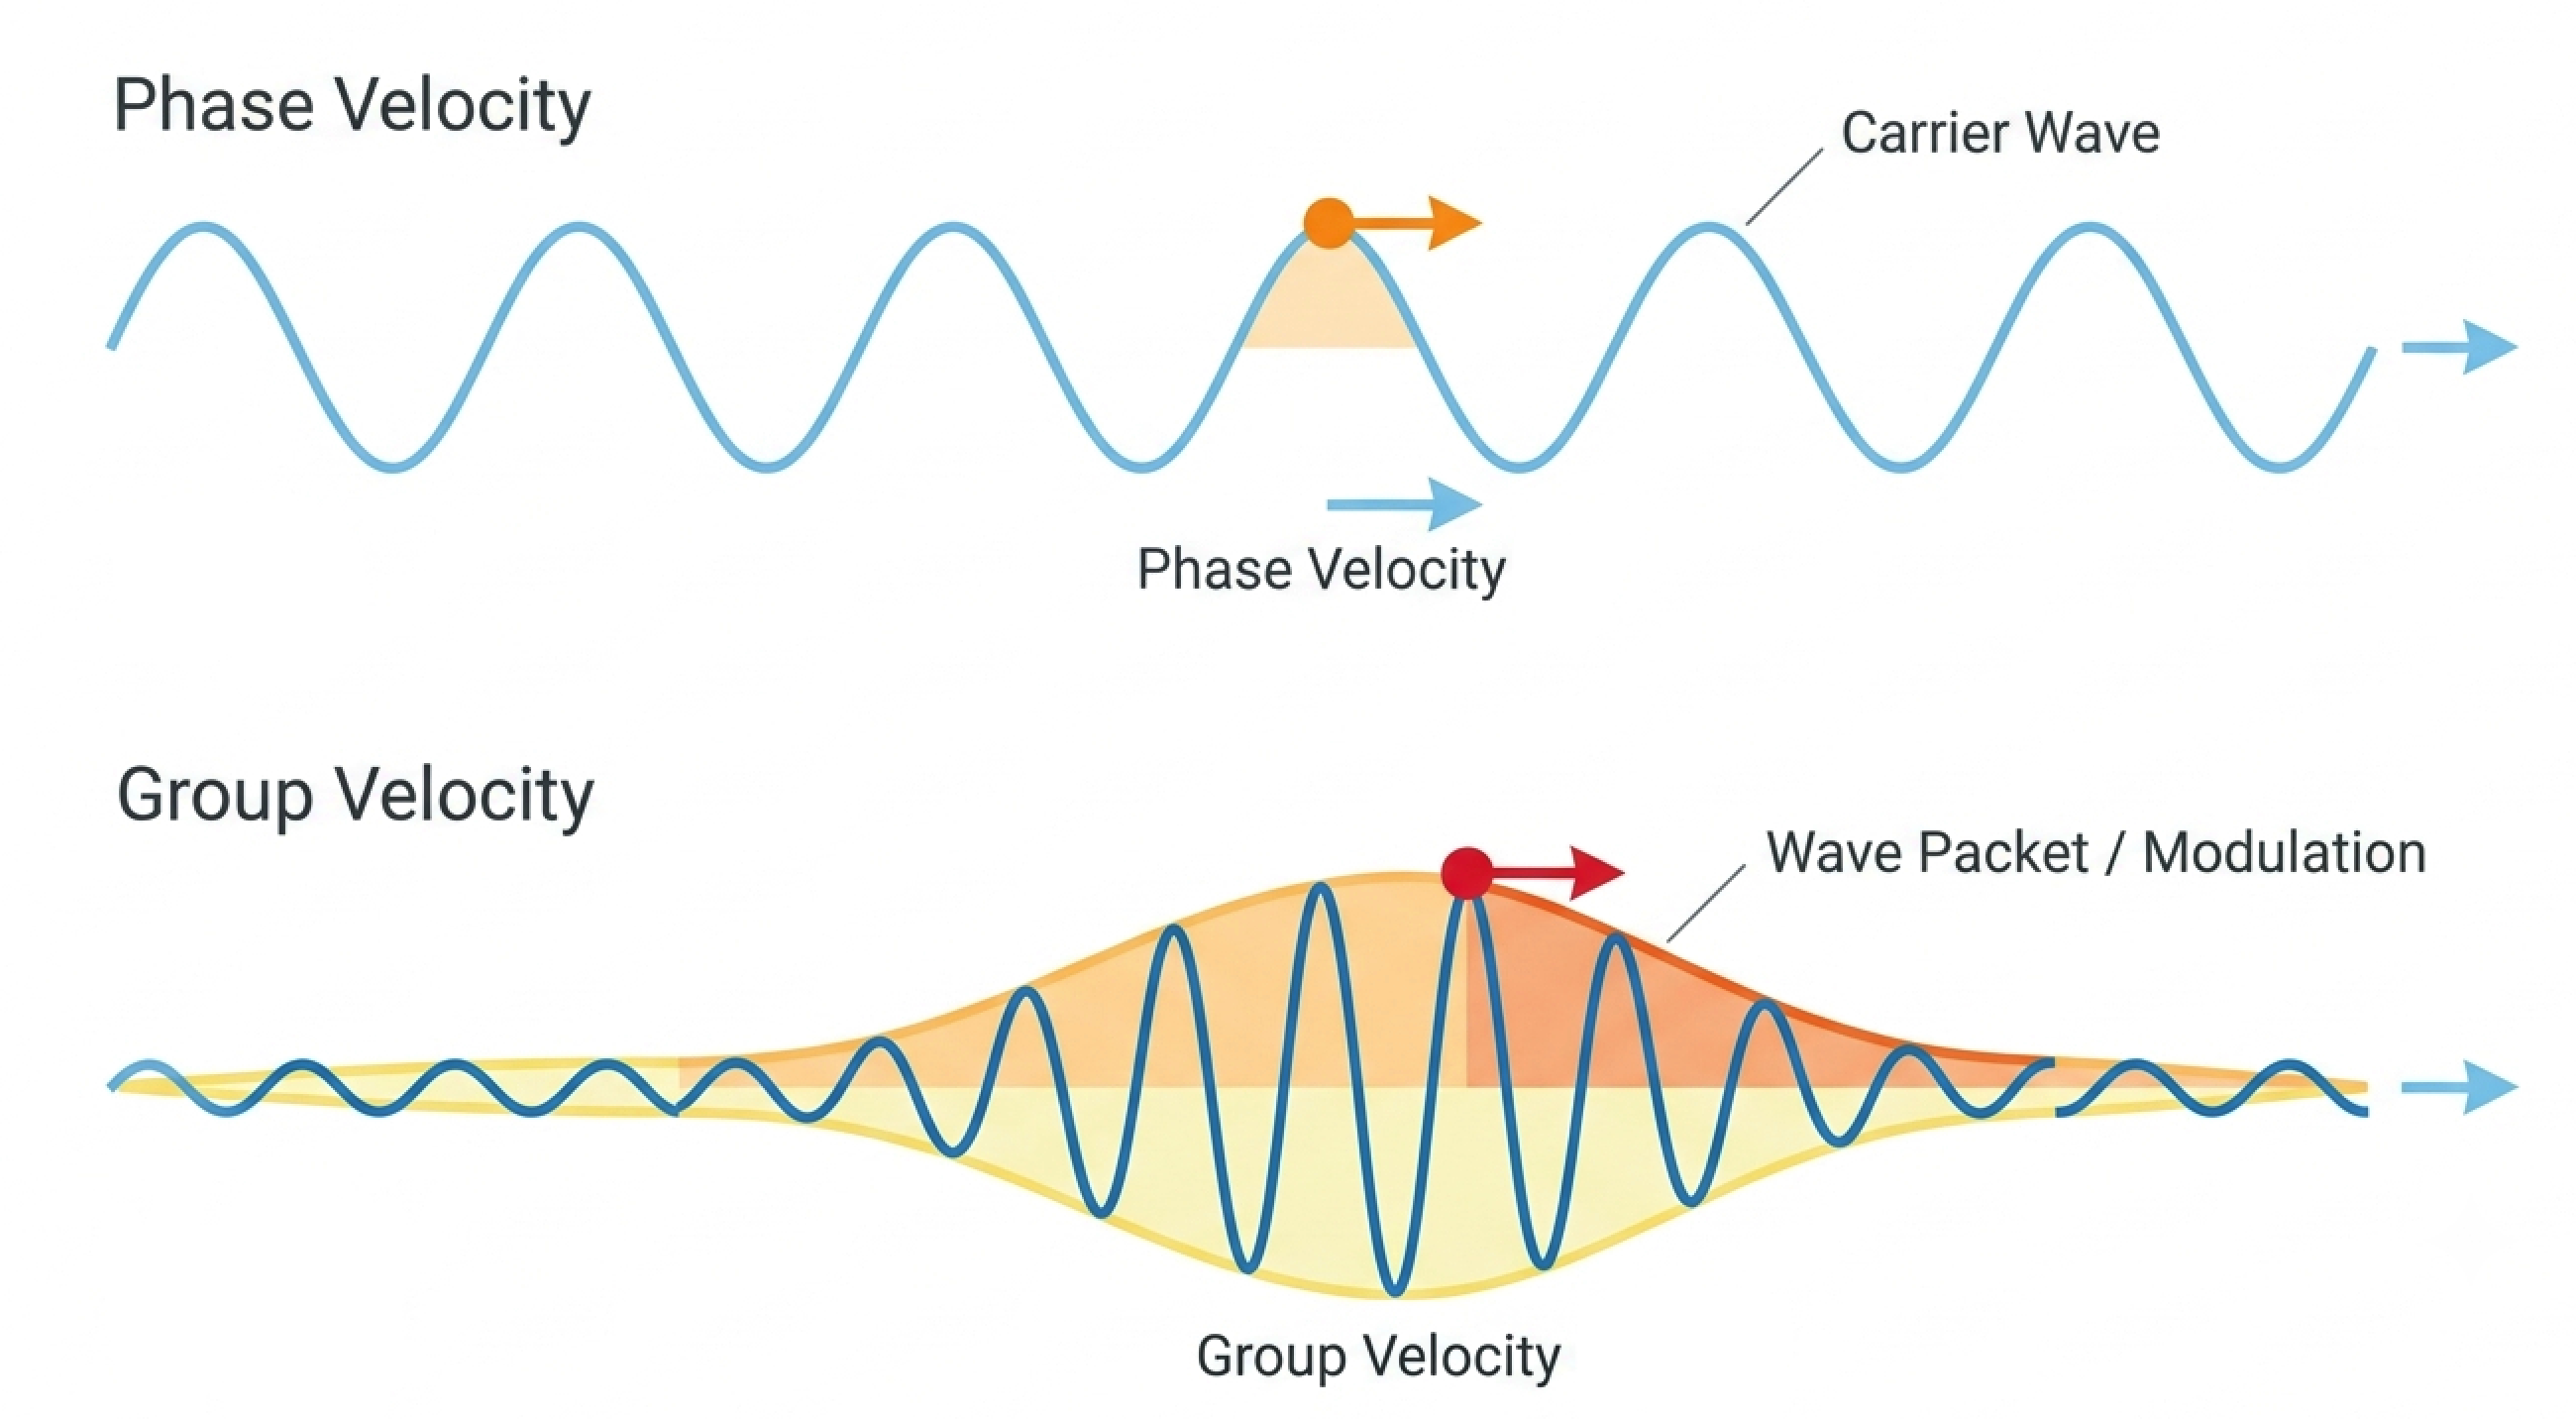
\includegraphics[height=5cm]{images/Fig2}
	\caption{Phase velocity vs Group velocity}
\end{figure}

\subsection{Time-Dependent Schrödinger Equation}
The derivation starts with the standard wave equation 
\begin{equation}
	\nabla^2 \Psi = \frac{1}{v^2} \frac{\partial^2 \Psi}{\partial t^2}
\end{equation}
where $\Psi$ is an arbitrary function of a physical quantity relevant to propagation of a wave(shape of a wave), $v$ is a phase velocity of wave, $ \nabla^2$ is called Laplacian and is defined as
\begin{equation}
	\nabla^2 \equiv \frac{\partial^2}{\partial x^2} + \frac{\partial^2}{\partial y^2} + \frac{\partial^2}{\partial z^2}
\end{equation}

\begin{figure}[h!]
	\centering
	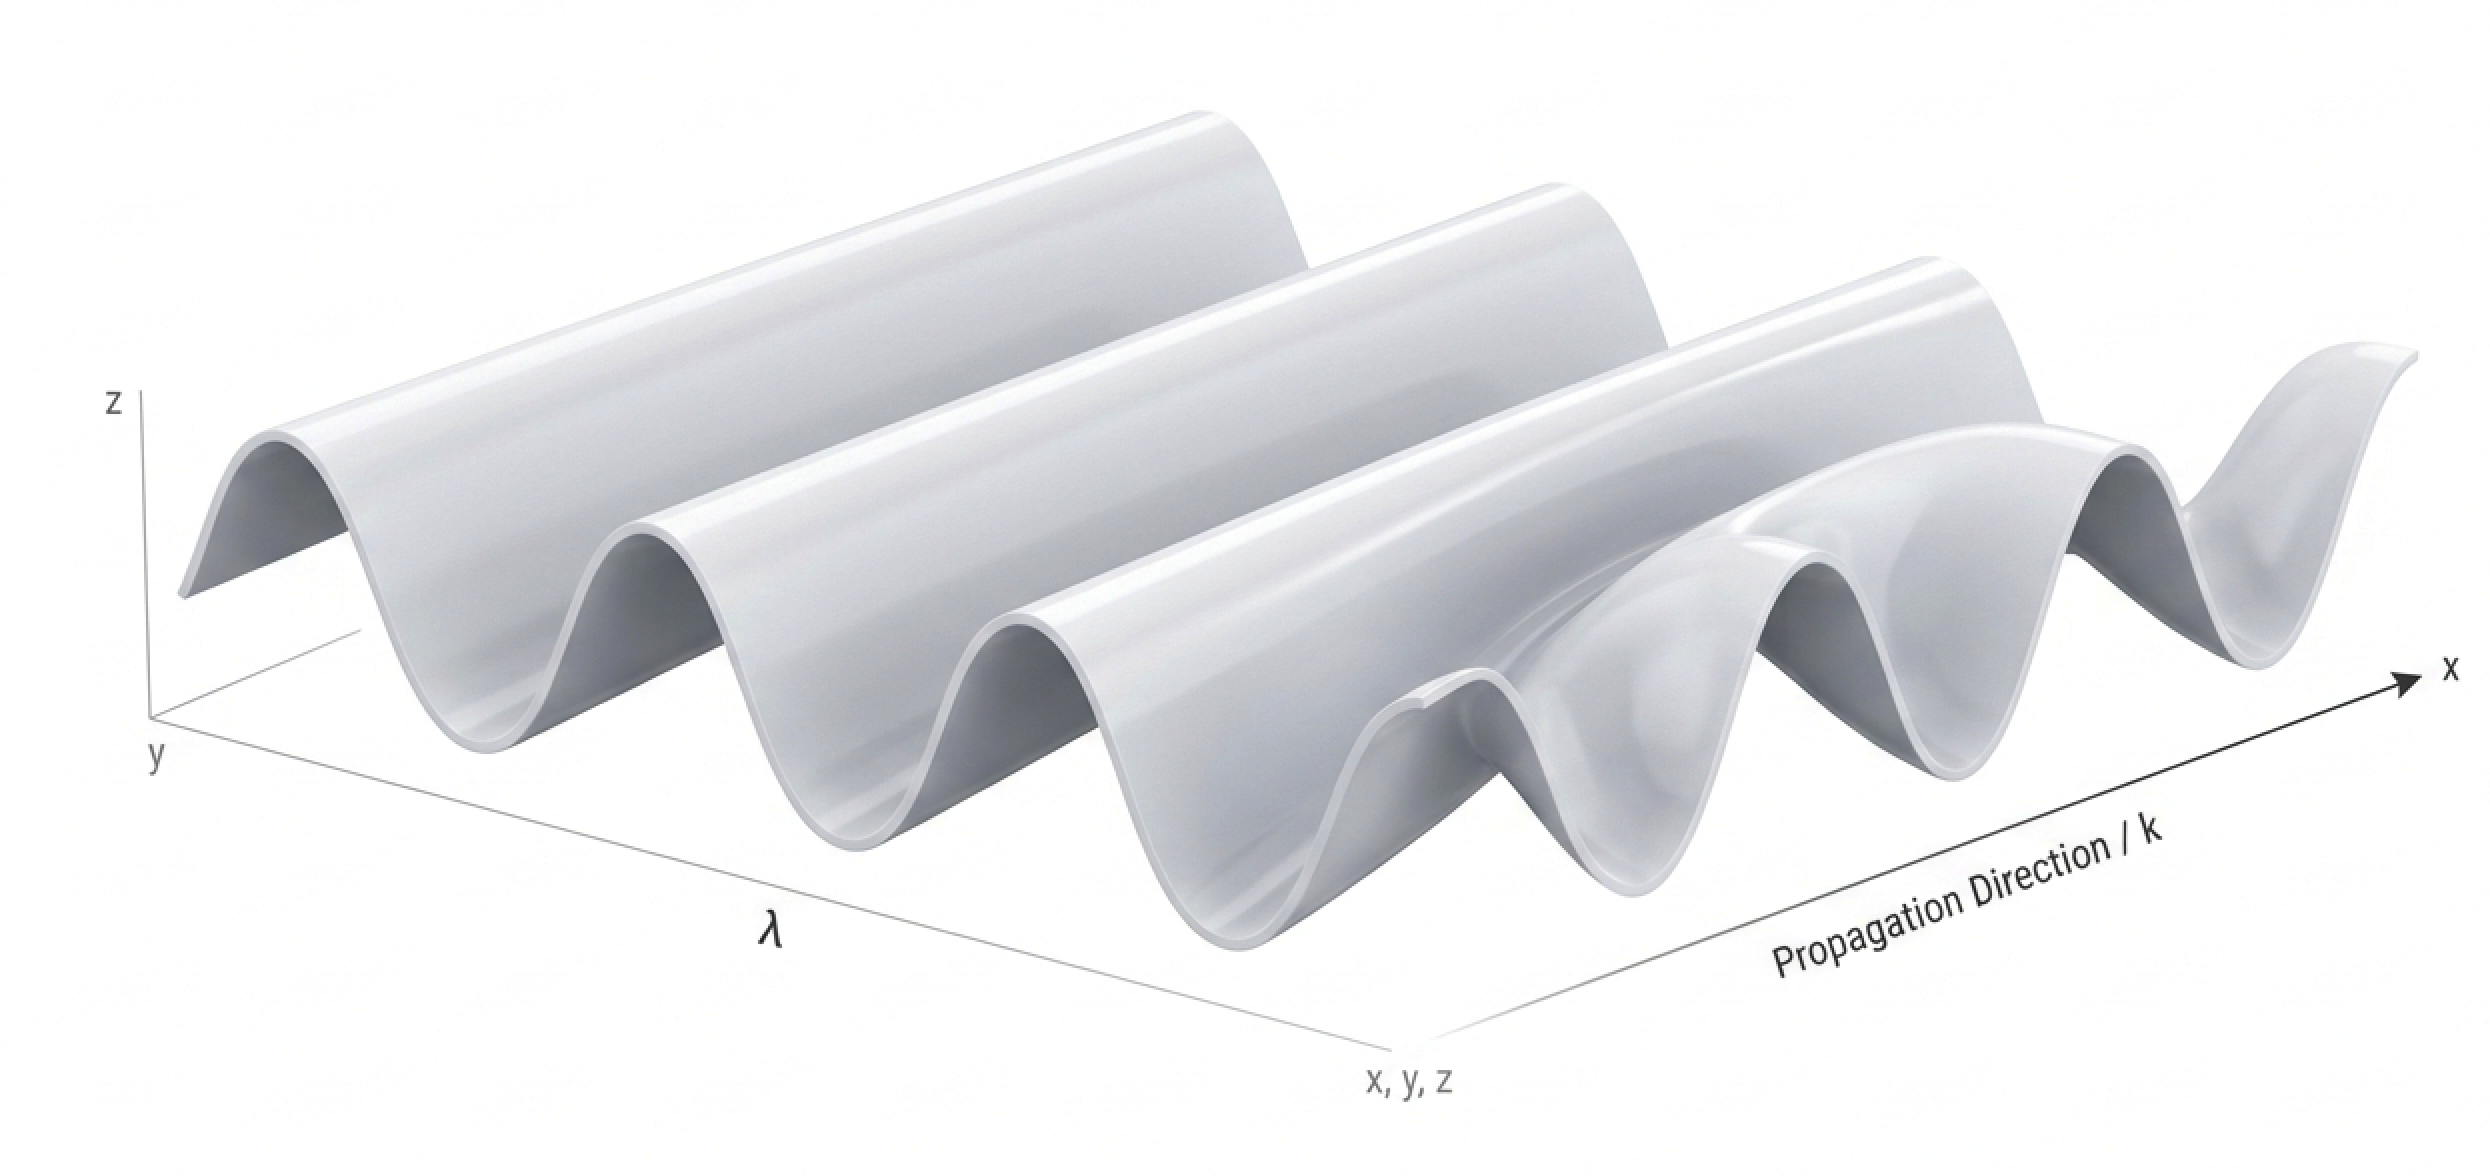
\includegraphics[width=7.5cm]{images/Fig3}
	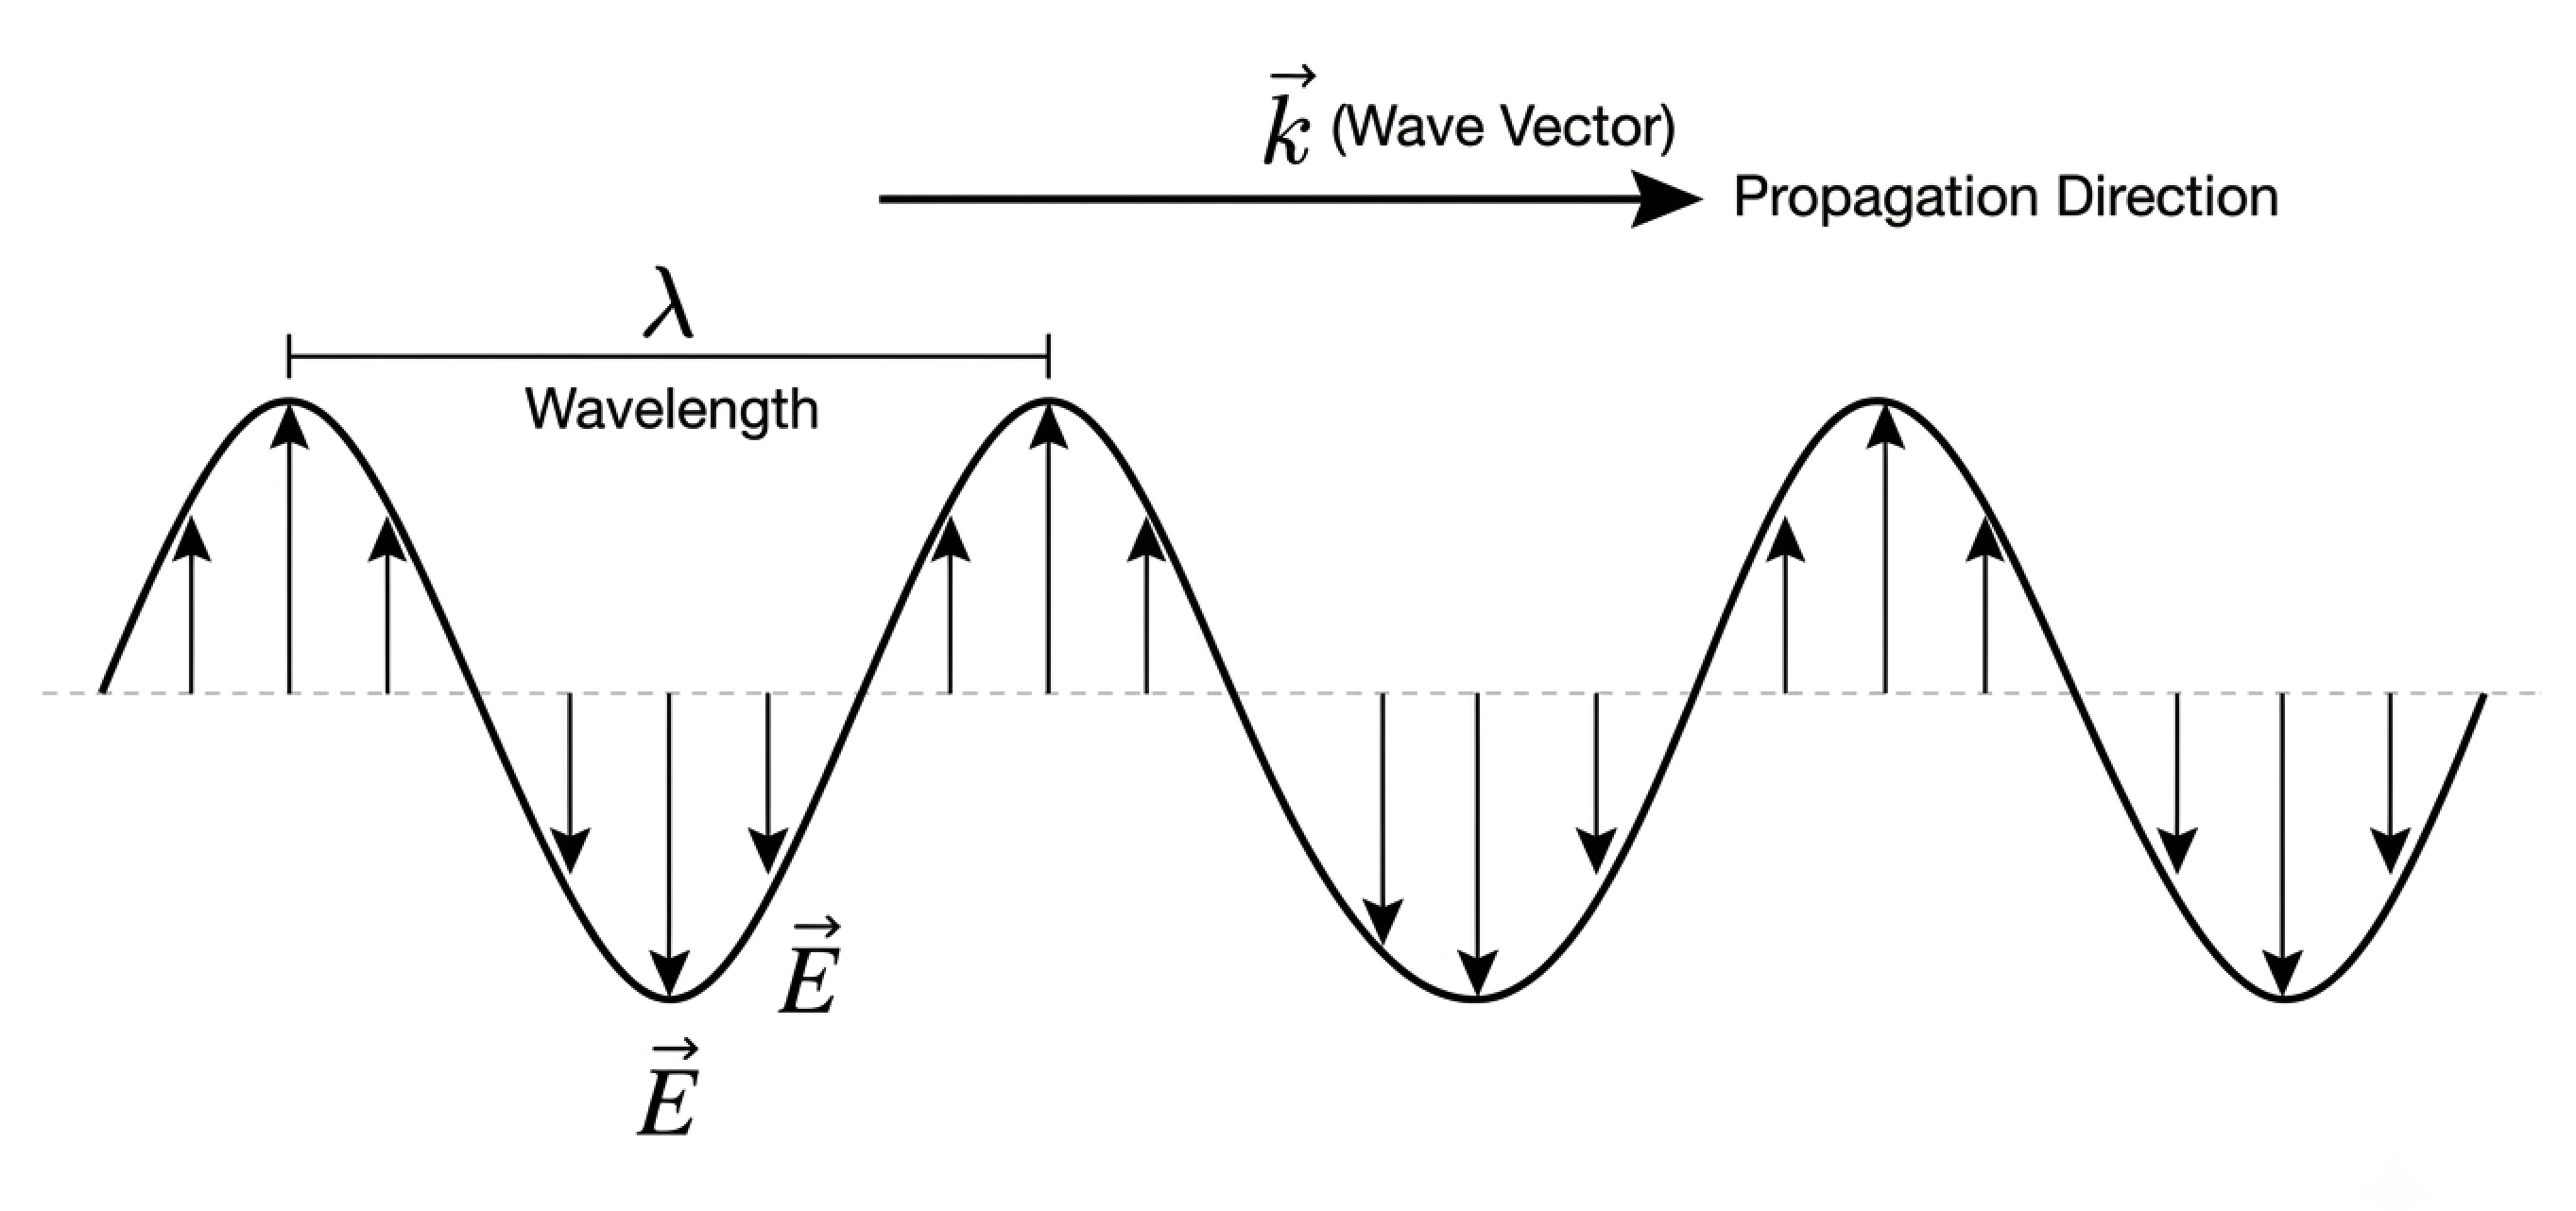
\includegraphics[width=7.5cm]{images/Fig4}
	\caption{Plane waves in two and three dimensions}
\end{figure}

One of the special solutions for wave equation is called a plane wave and its expressed as
\begin{equation}
	\Psi = \Psi_0 e^{i(k \cdot x - \omega t)} = \Psi_0 [ \cos (k \cdot x - \omega t) + i \sin (k \cdot x - \omega t) ]
\end{equation}
where $x$ denotes a position vector of a three-dimensional Cartesian coordinate. By applying de Broglie and Einstein’s relations, this is converted into a matter wave representing a particle:
\begin{equation} \label{eq:8}
	\Psi = \Psi_0 e^{i(\frac{p}{h} \cdot x - \frac{E}{h} t)}, \quad 
	p = \begin{pmatrix} e_1 \; e_2 \; e_3 \end{pmatrix} \begin{pmatrix} p_x \\ p_y \\ p_z \end{pmatrix}
\end{equation}
taking partial differentiation with respect to $x$ we obtain
\begin{equation}
	\frac{\partial \Psi}{\partial x} = \frac{i}{\hbar} p_x \Psi_0 e^{i(\frac{p}{h} \cdot x - \frac{E}{h} t)} = \frac{i}{\hbar} p_x \Psi \quad \Rightarrow \quad
	\frac{\hbar}{i} \frac{\partial \Psi}{\partial x} = p_x \Psi
\end{equation}
Similarly we have
\begin{equation}
	\frac{\hbar}{i} \frac{\partial \Psi}{\partial y} = p_y \Psi \quad \text{and} \quad \frac{\hbar}{i} \frac{\partial \Psi}{\partial z} = p_z \Psi
\end{equation}
Taking partial differentiation once more 
\begin{equation}
	\frac{\partial^2 \Psi}{\partial x^2} = (\frac{i}{\hbar} p_x)^2 \Psi_0 e^{i(\frac{p}{h} \cdot x - \frac{E}{h} t)} = - \frac{1}{\hbar^2} p_x^2 \Psi \quad \Rightarrow \quad
	- \hbar^2 \frac{\partial^2 \Psi}{\partial x^2} = p_x^2 \Psi
\end{equation}
Similarly we have
\begin{equation}
	- \hbar^2 \frac{\partial^2 \Psi}{\partial y^2} = p_y^2 \Psi \quad \text{and} \quad - \hbar^2 \frac{\partial^2 \Psi}{\partial z^2} = p_z^2 \Psi
\end{equation}
So if we summing both sides of these 3 equation and then dividing by $2m$ ($m$ is the mass of a particle), we have
\begin{equation} \label{eq:13}
	- \frac{\hbar ^ 2}{2m} \nabla^2 \Psi - \frac{p^2}{2m} \Psi
\end{equation}

Now lets get back to equation (\ref{eq:8}) and this time taking partial differentiation with respect to $t$, we obtain
\begin{equation} \label{eq:14}
	\frac{\partial \Psi }{\partial t} = - \frac{i}{\hbar} E \Psi_0 e^{i(\frac{p}{h} \cdot x - \frac{E}{h} t)} = - \frac{i}{\hbar} E \Psi \quad \Rightarrow \quad 
	i \hbar \frac{\partial}{\partial t} = E \Psi
\end{equation}
If we subtract (\ref{eq:13}) and (\ref{eq:14}) we get
\begin{equation} \label{eq:15}
	i \hbar \frac{\partial \Psi}{\partial t} + \frac{\hbar ^2}{2m} \nabla^2 \Psi = (E - \frac{p^2}{2m}) \Psi
\end{equation}
Comparing these equations we find out that momentum $p$ becomes the operator $ \frac{\hbar}{i} \nabla$ and energy $E$ becomes the operator $ i \hbar \frac{\partial}{\partial t}$. Now if we substituting these operators into the classical energy conservation relation (Total energy = Kinetic energy + Potential energy) we have
\begin{equation}
	E = \frac{p^2}{2m} + V
\end{equation}
So now lets rewrite the equation (\ref{eq:15})
\begin{equation} \label{eq:TDSE}
	i \hbar \frac{\partial \Psi}{\partial t} + \frac{\hbar ^ 2}{2m} \nabla^2 \Psi = V \Psi \quad \Rightarrow \quad
	(- \frac{\hbar ^ 2}{2m} \nabla^2 + V) \Psi = i \hbar \frac{\partial \Psi}{\partial t}
\end{equation}
This is the Time-Dependent Schrödinger Equation (TDSE), a fundamental equation of quantum mechanics. 

If we defind a following Hamiltonian operator $H$ (the sum of two components, the kinetic energy and the potential energy of a quantum system) as 
\begin{equation}
	H \equiv - \frac{\hbar^2}{2m} \nabla^2 + V 
\end{equation}
Then we have a shorthand representation such that
\begin{equation}
	H \Psi = i \hbar \frac{\partial \Psi}{\partial t}
\end{equation}
Since we want to associate the wave function with a single particle, it is reasonable to require the probability to find the electron anywhere in space to be exactly equal to one. Since this may not be the case for all $\Psi$, we introduce a normalization condition:
\begin{equation}
	\int_{- \infty}^{\infty} | \Psi (x,t) |^2 dx = 1
\end{equation}
The normalization thus imposes a condition on the wave function, the wave function must be a square integrable function.

\subsection{Time-Independent Schrödinger Equation}
In (\ref{eq:TDSE}) $\Psi$ is a function of $x$ and $t$. Suppose that a potential $V$ depends only upon $x$ and seperation of variables can be done with $\Psi$ function ($\Psi(x,t) = \phi(x) \xi(t)$). By substituting these functions into the Time-Dependent Schrödinger Equation, we have
\begin{equation}
	- \frac{\hbar^2}{2m} \nabla^2 \phi(x) \xi(t) + V(x) \phi(x) \xi(t) = i \hbar \phi(x) \frac{\partial \xi(t)}{\partial t}
\end{equation}
Now we will dividing the entire equation by $\phi(x) \xi(t)$
\begin{equation}
	\frac{- \frac{\hbar^2}{2m} \nabla^2 \phi(x)}{\phi(x)} + V(x)  = \frac{i \hbar \frac{\partial \xi(t)}{\partial t}}{\xi(t)}
\end{equation}
Since now the left hand side is only dependent on $x$ and the right hand side only on $t$, both sides must be equal to a constant, which is defined as the total energy$E$, and we can now solve each side independently
\begin{equation}\label{eq:TISE}
	H \phi(x) = E \phi(x)
\end{equation}
\begin{equation}
	\begin{aligned}
	& i \hbar \frac{\partial \xi(t)}{\partial t} = E \, \xi(t) 
	\quad \Rightarrow \quad \frac{d \xi(t)}{\xi(t)} = \frac{E}{i \hbar} \, dt 
	\quad \Rightarrow \quad \int \frac{d \xi}{\xi} = \frac{E}{i \hbar} \int dt \\
	& \quad \Rightarrow \quad \ln \frac{\xi(t)}{\xi(0)} = \frac{E t}{i \hbar} 
	\quad \Rightarrow \quad \xi(t) = \xi(0)\, \exp\!\left(-\frac{iEt}{\hbar}\right)
\end{aligned}
\end{equation}
The Time-Independent Schrödinger Equation (TISE)(\ref{eq:TISE}), is an eigenvalue problem where $E$ represents the energy eigenvalues and $\phi(x)$ represents the eigenfunctions (or stationary states) of the Hamiltonian operator. After solving the problem, we get a solution
\begin{equation}
	\Psi(x,t) = \phi(x) \exp\!\left(-\frac{iEt}{\hbar}\right)
\end{equation}

\section{Classical numerical methods for Schrödinger equation}
Classical numerical methods for solving the Schrödinger equation work by turning a continuous problem into a form that can be handled by a computer. Some common methods include finite difference and finite element methods, which divide space into small pieces and approximate derivatives. Spectral methods, such as Fourier, Chebyshev, and B-spline methods, instead represent the solution using combinations of known functions. Other useful approaches include the split-step Fourier method and the Crank–Nicolson method, which are often used to simulate how a system changes over time. Monte Carlo methods can also be used, especially for more complex or higher-dimensional problems.

For time-dependent Schrödinger equations, methods like Crank–Nicolson, implicit–explicit schemes, and operator splitting are popular because they are stable and work well for step-by-step time evolution. On the other hand, time-independent problems are usually solved using matrix diagonalization, variational methods, or Monte Carlo techniques to find energy levels and corresponding wave functions.

\subsection{Finite Difference Methods}
Finite Difference Methods (FDM) are numerical techniques used to approximate solutions to differential equations by discretizing the equations in both time and space. The continuous derivatives in the equations are replaced with finite difference approximations, which transform the problem into a system of algebraic equations that can be solved computationally. FDM is widely used to solve both time-dependent and time-independent forms of the Schrödinger equation.

\subsubsection{Discretizing the Domain}
Discretizing the domain transforms the continuous space and time where the wave function $\Psi (x,t)$ exists into a finite set of specific points called a mesh or grid, because computers cannot handle an infinite continuum of points.

The spatial domain is divided into equally spaced grid points defined as 
\begin{equation}
	x_j = j \Delta x \; ; \quad j = 0, 1, 2, \cdots , N
\end{equation}
where $\Delta x$ is the spatial step size and determines the resolution of the numerical approximation, with smaller values generally leading to higher accuracy at the expence of increased computaional cost.

Similarly, the time domain is divided into discrete time levels. The time points are defined as 
\begin{equation}
	t_n = n \Delta t \; ; \quad n = 0, 1, 2, \cdots
\end{equation}
where $\Delta t$ is the time step size and used to evolve the solution from one moment to the next.

After discretization, the continuous wave function $\Psi (x,t)$ is replaced by discrete values evaluated at the grid points. The value of the wave function at position $x_j$ and time $t_n$ is denoted by
\begin{equation}
	\Psi_j^n \approx \Psi (x_j, t_n)
\end{equation}
At any time step $n$ the entire spatial state can be treated as a vector 
\begin{equation}
	U^n = \begin{pmatrix} \Psi_0^n \\ \Psi_1^n \\ \vdots \\ \Psi_N^n \end{pmatrix}
\end{equation}
which represents the numerical state of the system at that particular time.

\subsubsection{Approximating the Schrödinger Equation}
After discretizing the computational domain, the next step in the finite difference method is to approximate the derivatives appearing in the Schrödinger equation. Since numerical algorithms cannot directly evaluate continuous derivatives, these derivatives are replaced by algebraic expressions involving values of the wave function at neighboring grid points. This transformation converts the differential equation into a system of algebraic equations that can be solved using a computer.

The kinetic energy term in the Schrödinger equation contains the second spatial derivative of the wave function. A commonly used approximation is the second-order centered finite difference formula
\begin{equation}
	\frac{\partial^2 \Psi}{\partial x^2} \approx \frac{\Psi_{j+1}^n - 2 \Psi_j^n + \Psi_{j-1}^n}{\Delta x^2}
\end{equation}
This approximation is second-order accurate, meaning that the truncation error is proportional to $O(\Delta x^2)$. As a resault, reducing the grid spacing improves the accuracy of the numerical solution.

The time derivative of the wave function can also be approximated using finite differences. One of the simplest approximations is the forward difference scheme
\begin{equation}
	\frac{\partial \Psi }{\partial t} \approx \frac{\Psi_j^{n+1} - \Psi_j^n}{\Delta t}
\end{equation}
For improved accuracy, central difference approximations may be employed. In this case, the derivative is approximated by
\begin{equation}
	\frac{\partial \Psi }{\partial t} \approx \frac{\Psi_j^{n+1} - \Psi_j^{n-1}}{2 \Delta t}
\end{equation}

\subsubsection{Implementation Strategies}
After discretization and derivative approximation, the finite difference equations must be solved using an appropriate numerical strategy. Several implementation techniques have been developed depending on the type of Schrödinger equation being considered and the desired numerical properties, such as stability, efficiency, and accuracy.

\begin{itemize}
	\item 
	The Method of Lines (MoL):
\end{itemize}
In this method, only the spatial derivatives(the Laplacian) are discretized using finite differences, while the time variable remains continuous. As a result, the Schrödinger equation is transformed into a system of coupled ordinary differential equations (ODEs) where $\hbar = m = 1$
\begin{equation}
	 \frac{d \Psi}{dt} = \frac{i}{2} \left[ \frac{\Psi_{j+1}^n - 2 \Psi_j^n + \Psi_{j-1}^n}{\Delta x^2} \right] - i V \Psi(t) \quad \Rightarrow \quad
	 \frac{d \Psi}{dt} = S(\Psi)
\end{equation}
Time evolution is then performed using an explicit third-order Runge–Kutta (RK3) scheme:
\begin{equation}
	k_1 = \Delta t S(\Psi ^n), \quad 
	k_2 = \Delta t S(\Psi ^n + \frac{1}{2} k_1), \quad 
	k_3 = \Delta t S(\Psi ^n + \frac{1}{2} k_2)
\end{equation}
\begin{equation}
	\Psi^{n+1} = \Psi^n + \frac{1}{6} k_1 +  \frac{2}{3} k_2 + \frac{1}{6} k_3
\end{equation}

\begin{itemize}
	\item 
	Imaginary Time Evolution (Wick Rotation):
\end{itemize}
Imaginary Time Evolution is a numerical technique commonly used to compute the stationary states of the Schrödinger equation, particularly the ground state. The method is based on the substitution $\tau = it$ where $t$ is the real time and $\tau$ is the imaginary time. This transformation, often referred to as a Wick rotation, converts the time-dependent Schrödinger equation into a diffusion-type equation (a partial differential equation that describes how a physical quantity spreads or smooths out over time due to diffusion-like processes: $\frac{\partial u}{\partial t} = D \nabla^2 u$).
\begin{equation}
	\frac{\partial}{\partial t} = i \frac{\partial}{\partial \tau} \quad \Rightarrow \quad
	\frac{\partial \Psi}{\partial \tau} = \frac{\hbar}{2m} \nabla^2 \Psi - \frac{V}{\hbar} \Psi 
\end{equation}
Notice that this has the same structure as the diffusion equation. The Laplacian causes the wavefunction to become smoother over imaginary time, while the potential term acts as a source or sink.

If the initial wave function is expressed as a linear combination of the eigenfunctions of the Hamiltonian we have
\begin{equation}
	\Psi(x, \tau) = \sum_{n} c_n \phi_n (x) e^{-E_n \tau}
\end{equation}
where $\phi_n(x)$ are the eigenfunctions, $E_n$ are the corresponding energy eigenvalues, and $c_n$ are expansion coefficients, each component decays exponentially as the imaginary time increases. As $ \tau \to \infty $, $e^{-(E_n - E_0) \tau} \to 0$ for $n > 0$. so only the ground state remains $\Psi (\tau) \approx c_0 \phi_0 e^{E_0 \tau}$

\begin{itemize}
	\item 
	Boundary Management:
\end{itemize}
For a finite computational domain $\Omega = [a,b]$, Dirichlet boundary conditions impose homogeneous constraints on the wave function $\Psi(a,t) = \Psi(b,t) = 0$. his corresponds to an infinite potential barrier outside $\Omega$, i.e.
\begin{equation}
	V(x) = 
	\begin{cases} 
		V(x) & \text{if } x \in \Omega \\
		\infty & \text{if } x \notin \Omega 
	\end{cases}
\end{equation}
To prevent waves from reflecting off the grid edges back into the simulation, an imaginary potential $\mathfrak{Im}(V)$ is added to the Hamiltonian and modifies the continuity equation for probability density $\rho = \Psi \Psi^* = |\Psi|^2$. If $\mathfrak{Im}(V)$ is negative, it acts as a sink, causing the probability density to decay as it enters the sponge region.
\begin{equation}
	\frac{\partial \rho}{\partial t} + \nabla \cdot J = 2 \rho \mathfrak{Im}(V)
\end{equation}
A typical smooth absorber is constructed using a hyperbolic tangent profile:
\begin{equation}
	\mathfrak{Im}(V) = - \frac{1}{2} V_0 \left\{ 2 + \tanh \left( \frac{(r - r_c)}{\delta}  \right) - \tanh (\frac{r_c}{\delta}) \right\}
\end{equation}
 where $V_0$ is the depth of the well, $r_c$ is the radius where the sponge starts, and $\delta$ is the transition width

For unbounded domains (infinite space), non-local boundary conditions allow waves to exit the domain as if the grid were infinite. These conditions are non-local in time, meaning the value at the boundary at time $t$ depends on the history of the wave function at that point. For a potential $V_-$ outside the boundary at $x=0$, the boundary condition takes the form
\begin{equation}
	\partial_x \Psi(0,t) = \sqrt{\frac{2}{\pi}} e^{-i\pi/4} e^{-iV_- t} \frac{d}{dt} \int_0^t \frac{\Psi(0,\tau)e^{iV_- \tau}}{\sqrt{t-\tau}}\, d\tau.
\end{equation}

\subsection{Finite Element Methods}
The Finite Element Method (FEM) is a numerical technique that approximates the solution by dividing the domain into a collection of small subdomains called finite elements, and finding an approximate solution using locally defined basis functions. Unlike the Finite Difference Method (FDM), which approximates derivatives directly at discrete grid points, FEM transforms the governing differential equation into its weak (variational) form before discretization. This formulation provides greater flexibility for handling complex geometries, irregular meshes and variable material properties.

\subsubsection{Discretizing the Domain}
Domain discretization is the first step. Let $\Omega \subset \mathbb{R}^d$ where $d=1,2,3$ denote the domain. Such that
\begin{equation}
	\bar{\Omega} = \bigcup_{e=1}^{m} \Omega_e
\end{equation}
where $\Omega_e$ represents the $e$th finite element and $m$ is the total number of elements. The interiors of any two distinct elements satisfy $\Omega_i \bigcap \Omega_j = \emptyset \quad i \neq j$ ensuring that the mesh completely covers the computational domain without overlap.  In 1D, elements are intervals $[ x_j, x_{j+1}]$, in 2D they are typically triangles or quadrilaterals and in 3D they are tetrahedra or hexahedra (bricks). Elements are interconnected at a finite number $N$ of nodal points $ \{ x_k \}_{k = 1}^N$ situated on their boundaries (and sometimes interiors)

The accuracy of the approximation depends strongly on the quality of the computational mesh. The mesh size is defined by 
\begin{equation}
	h = \max_{\Omega \in \tau_h} diam(\Omega) ; \quad diam(\Omega) = \max_{x,y \in \Omega} || x - y ||
\end{equation}
where $diam(\Omega)$ is the diameter  of element $\Omega$ in partition $\tau_h$. as the mesh is refined $h \to 0$ the finite element solution converges toward the exact solution. for convergence and numerical stability, the mesh is generally required to satisfy quasi-uniformity conditions, preventing excessively distorted elements. In practical applications involving irregular geometries, unstructured meshes are commonly used because they have better geometric flexibility than structured grids.

After choosing the mesh, a finite-dimensional approximation space is defined. For the Schrödinger equation, this space is typically chosen as $V_h \subset H^1 (\Omega)$ (also known as Sobolev space) where $V_h = span \{ N_1, N_2, \cdots , N_N \}$ (also called shape functions) and each basis function is associated with a single mesh node.
The shape functions satisfy the interpolation property:
\begin{equation}
	N_i (x_j) = \delta_{ij} = 
		\begin{cases} 
		1 & \text{if } i = j \\
		0 & \text{if } i \neq j 
	\end{cases}
\end{equation}
This property guarantees that the nodal coefficients correspond directly to the values of the approximate solution at the mesh nodes. Furthermore, the basis functions satisfy the partition of unity:
\begin{equation}
	\sum_{i=1}^N N_i(x) = 1 ; \quad \forall x \in \Omega
\end{equation}

The continuous wave function is approximated by a finite-dimensional expansion over the chosen basis functions
\begin{equation}
	\Psi (x,t) \approx \Psi_h (x,t) = \sum_{i=1}^N N_i(x) \Psi_i (t)
\end{equation}
where $N_i(x)$ are the finite element basis functions and $\Psi_i (t)$ are the unknown time-dependent nodal coefficients representing the state of the system at node $i$. This discretization effectively transforms the TDSE into a system of ordinary differential equations in time which can be solved as a system of algebraic equations at each time step.

\subsubsection{Weak Solution Formulation}
Instead of requiring the solution to satisfy the Schrödinger equation pointwise, the equation is reformulated as an integral identity over the computational domain. This approach reduces the differentiability requirements on the solution, making it possible to approximate the wave function using piecewise polynomial basis functions.

Let $\Omega \subset \mathbb{R}^{d} (d=1,2,3)$ denote the computational domain with boundary $ \partial\Omega$. The unknown wave function is sought in the Sobolev space
\begin{equation}
	H_0^1 (\Omega) = \{ u \in H^1 (\Omega) : u = 0 \quad \text{on} \quad \partial \Omega \}
\end{equation}
which consists of square-integrable functions whose first weak derivatives are also square-integrable and which satisfy Dirichlet boundary conditions. To derive the weak formulation let $\chi \in H_0^1(\Omega)$ be an arbitrary complex-valued test function. The core principle is that if the TDSE is satisfied at every point in the domain $\Omega$, then the integral of the equation multiplied by any arbitrary test function must also be zero.

Consider the time-dependent Schrödinger equation
\begin{equation}
	i \hbar \frac{\partial\Psi}{\partial t} = - \frac{\hbar^2}{2m} \nabla^2 \Psi + V \Psi + f
\end{equation}
where $V(x)$ is the potential function and $f$ denotes a source term. Multiplying the equation by the complex conjugate of the test function $\overline{\chi}$ and integrating over the computational domain yields
\begin{equation} \label{eq:49}
	i \hbar \int_{\Omega} \frac{\partial \Psi}{\partial t} \overline{\chi} d \Omega = 
	- \frac{\hbar^2}{2m} \int_{\Omega} \nabla^2 \Psi \overline{\chi} d \Omega +
	 \int_{\Omega} V\Psi \overline{\chi} d \Omega +
	\int_{\Omega} f \overline{\chi} d \Omega
\end{equation}
We define the inner product as
\begin{equation}
	(u,v) = \int_{\Omega} u \overline{v} d \Omega
\end{equation}
The (\ref{eq:49}) equation can be written compactly as
\begin{equation}
	i \hbar (\Psi_t, \chi) = - \frac{\hbar^2}{2m} (\nabla^2 \Psi, \chi) + (V \Psi, \chi) + (f, \chi)	
\end{equation}
The Laplacian term contains second-order spatial derivatives so we will apply Green’s first identity 
\begin{equation}
	\int_{\Omega} \nabla^2 \Psi  \overline{\chi} d \Omega = - \int_{\Omega} \nabla \Psi \cdot \nabla \overline{\chi} d \Omega + \int_{\partial \Omega} \overline{\chi} \frac{\partial \Psi}{\partial n} d \Gamma
\end{equation}
where $\frac{\partial \Psi}{\partial n} = \nabla \Psi \cdot \mathbf{n}$ denotes the outward normal derivative on the boundary. Since the test functions satisfy $ \chi=0$ on $\partial \Omega$, the boundary integral vanishes and resulting in
\begin{equation}
	\int_{\Omega} \nabla^2 \Psi \overline{\chi} d \Omega = - \int_{\Omega} \nabla \Psi \cdot \nabla \overline{\chi} d \Omega
\end{equation}
the second-order derivative acting on the wave function is replaced by first-order derivatives acting on both the trial and test functions. This reduction in derivative order is the defining feature of the weak formulation.

Substituting the results of integration by parts back into the integral statement yields the Weak Solution Formulation:
Find $\Psi (\cdot, t) \in H_0^1(\Omega)$ such that
\begin{equation}
		i \hbar(\Psi_t,\chi) = a(\Psi, \chi) + (f, \chi) ; \quad \forall \chi \in H_0^1(\Omega)
\end{equation}
where $ a(\Psi,\chi) = \frac{\hbar^2}{2m} (\nabla \Psi,\nabla \chi) + (V\Psi,\chi)$ is the bilinear form representing the Hamiltonian components. This variational equation forms the mathematical basis for the finite element discretization of the Schrödinger equation.


\begin{thebibliography}{99}
	
	\bibitem{Hotta2020}
	S. Hotta, \emph{Mathematical Physical Chemistry: Practical and Intuitive Methodology}, 2nd ed. Singapore: Springer Singapore, 2020. doi: 10.1007/978-981-15-2225-3.
	
	\bibitem{Mezzetti2021}
	G. Mezzetti, \emph{Introduction to the Schr\"odinger Equation and an Application to the Stock Market}, Master's thesis, Luiss Guido Carli University, Rome, Italy, 2021. [Online]. Available: https://tesi.luiss.it/33247/. Supervisor: F. Gozzi.
	
	\bibitem{Becerril2008}
	R. Becerril, F. S. Guzm\'an, A. Rend\'on-Romero, and S. Valdez-Alvarado,  
	“Solving the time-dependent Schr\"odinger equation using finite difference methods,”  
	\emph{Revista Mexicana de F\'isica E}, vol. 54, no. 2, pp. 120--132, 2008.
	
	\bibitem{Sudiarta2007}
	I. W. Sudiarta and D. J. W. Geldart,  
	“Solving the Schr\"odinger equation using the finite difference time domain method,”  
	\emph{Journal of Physics A: Mathematical and Theoretical}, vol. 40, no. 8, pp. 1885--1900, 2007. doi: 10.1088/1751-8113/40/8/013.
	
	\bibitem{Han2007}
	H. Han,  
	“A finite-difference method for the one-dimensional time-dependent Schr\"odinger equation on unbounded domain,”  
	\emph{Journal of Computational and Applied Mathematics}, 2007. doi: 10.1016/j.cam.2006.10.038.
	
	\bibitem{Zienkiewicz2005}
	O. C. Zienkiewicz, R. L. Taylor, and J. Z. Zhu,  
	\emph{The Finite Element Method: Its Basis and Fundamentals}, 6th ed. Amsterdam: Elsevier Butterworth-Heinemann, 2005.
	
	\bibitem{EsenTasbozan2017}
	A. Esen and O. Tasbozan,  
	“Numerical solution of time fractional Schr\"odinger equation by using quadratic B-spline finite elements,”  
	\emph{Annales Mathematicae Silesianae}, vol. 31, no. 1, pp. 83--98, 2017. doi: 10.1515/amsil-2016-0015.
	
	\bibitem{FanQi2015}
	W. Fan and H. Qi,  
	“An efficient finite element method for the two-dimensional nonlinear time-space fractional Schr\"odinger equation on an irregular convex domain,”  
	\emph{Applied Mathematics and Computation}, vol. 259, pp. 12--26, 2015. doi: 10.1016/j.amc.2015.02.048.
	
	\bibitem{Gass1976}
	I. T. Gass,  
	“Solution of the Schr\"odinger wave equation in a space-time continuum by a finite element formulation,”  
	\emph{International Journal for Numerical Methods in Engineering}, vol. 10, no. 1, pp. 1--15, 1976. doi: 10.1002/nme.1620100102.
	
\end{thebibliography}























\section{PINN Method}

\subsection{Neural Networks}
The Artificial Neural Network (ANN) is a computational approach to modeling the biological neural 
network's structure and functionality. ANNs are made up of connected units known as neurons,
and these are organized in layers: there is an input layer, one or several hidden layers, and an output layer. 
A weight is assigned to each link, defining the strength of the information transmission across it.

In feedforward networks, information travels through successive layers from input to output,
passing first through hidden layers. In each node, information enters and is processed,
undergoing weighted addition and then nonlinear transformation with the use of an activation function. 
The training process involves modifying the network's parameters according to a loss function using algorithms 
for gradient descent such as backpropagation.

Neural networks are universal function approximators, meaning that, given enough training samples, 
they can approximate any continuous function. 
As a result of their capacity to discover intricate non-linear links between inputs and outputs, 
neural networks have found numerous applications in a variety of fields like image processing, text recognition, 
scientific computation, and the resolution of differential equations.
In the context of Physics-Informed Neural Networks (PINNs), neural networks are employed to 
approximate the solution of a differential 
equation while simultaneously satisfying the governing physical laws through additional c
onstraints incorporated into the loss function.[1]


Mathematically, a feed-forward neural network can be understood as a composition of several functions. Each layer transforms the output of the previous layer until the final output is produced. If the network has (L) layers, then the approximation can be written as

$$F_L \circ F_{L-1} \circ \cdots \circ F_1(t,x)$$


where each $(F_i)$ represents the transformation performed by the $(i)-th$ layer. This layered structure allows the network to build increasingly complex representations of the solution.


\begin{figure}[h]
	\centering
	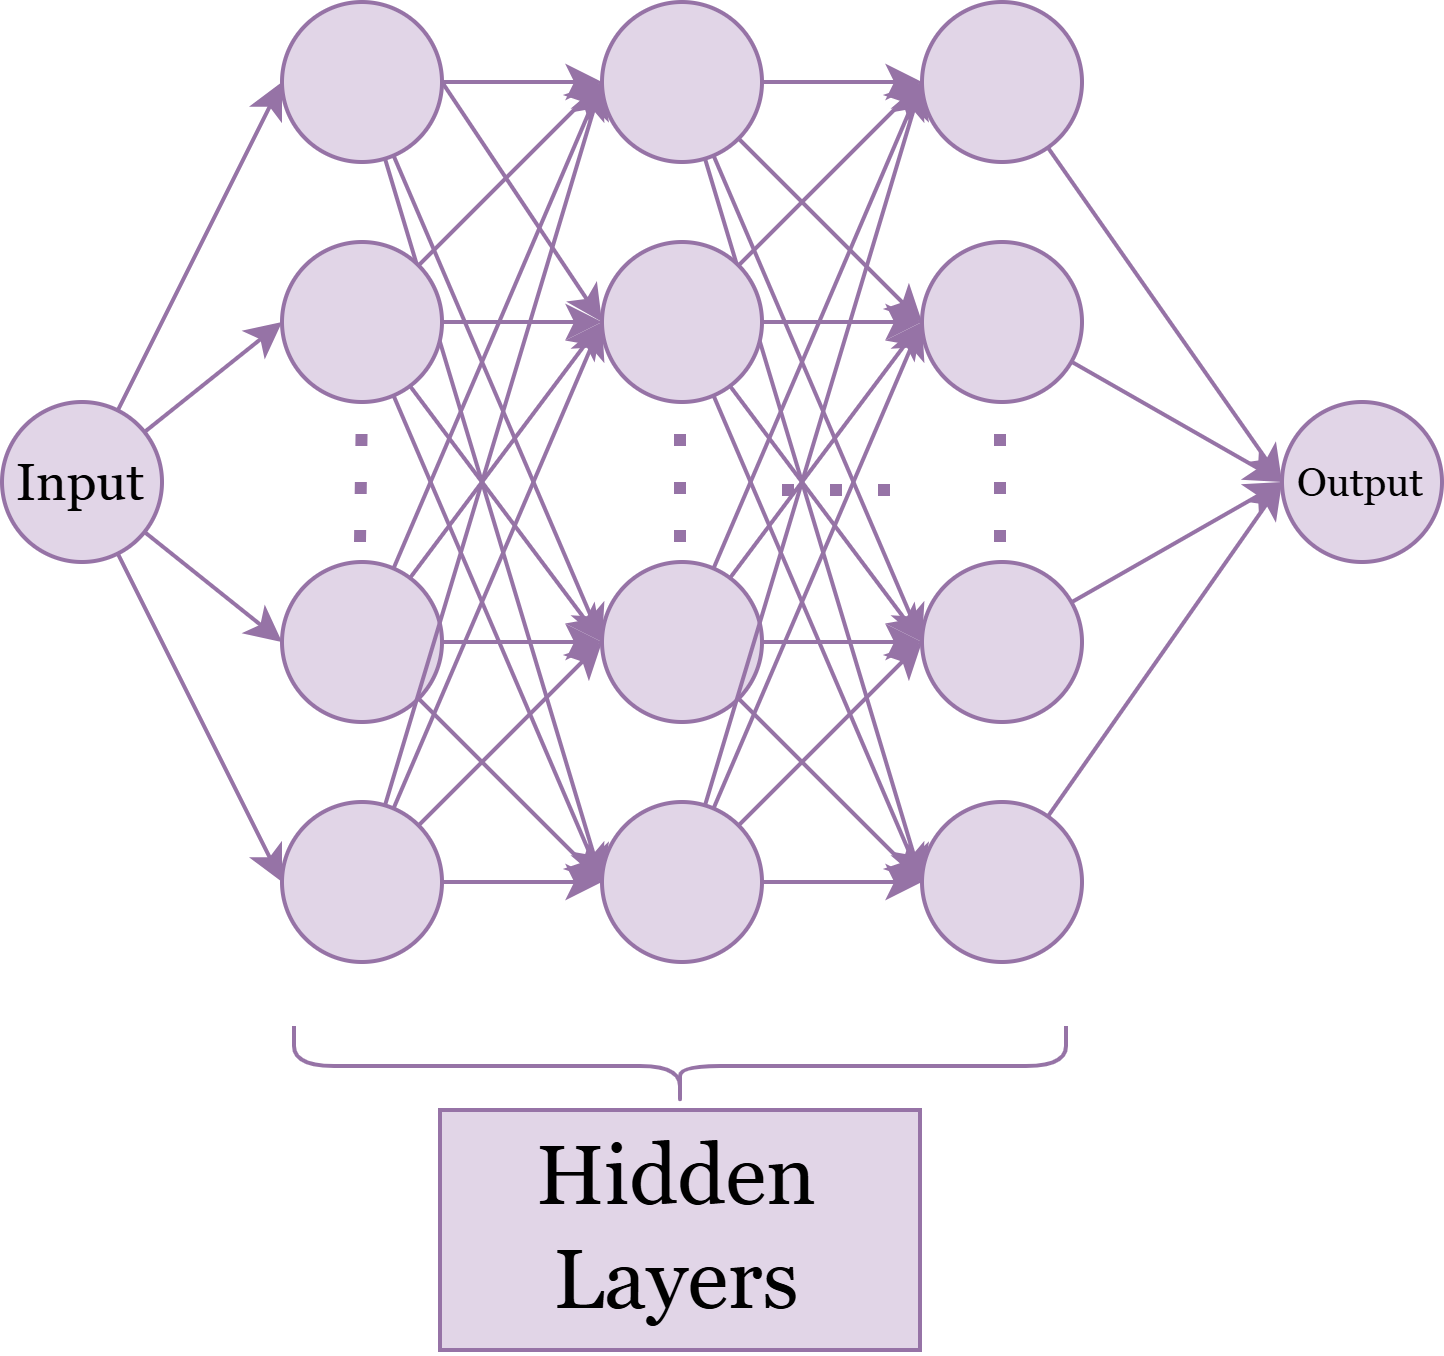
\includegraphics[width=.4\textwidth]{images/Neural_Network.png}
	\caption{Nerual Network}
	\label{fig:nn}
\end{figure}

\vspace{3in}

\subsection{PINNs}
The conventional neural network is trained with the help of data only. If we provide some data samples to 
the network, the network tries to minimize the error between the predicted output values and the observed
values. Though this methodology has produced very good results in many different scenarios, it needs plenty 
of data and does not ensure that the solution that is predicted by the model complies with the physical laws.

On the other hand, Physics-Informed Neural Networks (PINNs) combine the concept of a neural network with the 
physical laws governing the system. Unlike a standard neural network, which is trained using data only, 
a PINN is constrained by physical laws represented by a Partial Differential Equation (PDE). 
Here, the neural network is responsible for approximating the unknown solution $(u(t,x))$, whereas automatic
differentiation is used to calculate the necessary derivatives in the PDE.
For a general PDE of the form

\begin{equation}
	u_t + \mathcal{N}[u] = 0
\end{equation}



the neural network predicts the solution $(u(t,x))$. Using automatic differentiation, 
the derivatives $(u_t), (u_x), (u_{xx})$, and higher-order terms can be computed exactly with respect to the network inputs. 
These derivatives are then substituted into the governing equation to form a residual function

\begin{equation}
	f(t,x) = u_t + \mathcal{N}[u].
\end{equation}

In case the neural network adheres exactly to the physical law, then the residual 
(f(t,x)) is supposed to take the value of zero throughout the whole domain. 
Hence, there will be two components in the training process of a PINN. 
One is related to the data error while the other component relates to physics, 
which serves as an additional constraint.

A PINN may therefore be regarded as a neural network that makes use of both 
observation data as well as the principles of physics. The incorporation of 
such physical knowledge provides additional information for the network, 
which works as a regularization technique.



\begin{figure}[h]
	\centering
	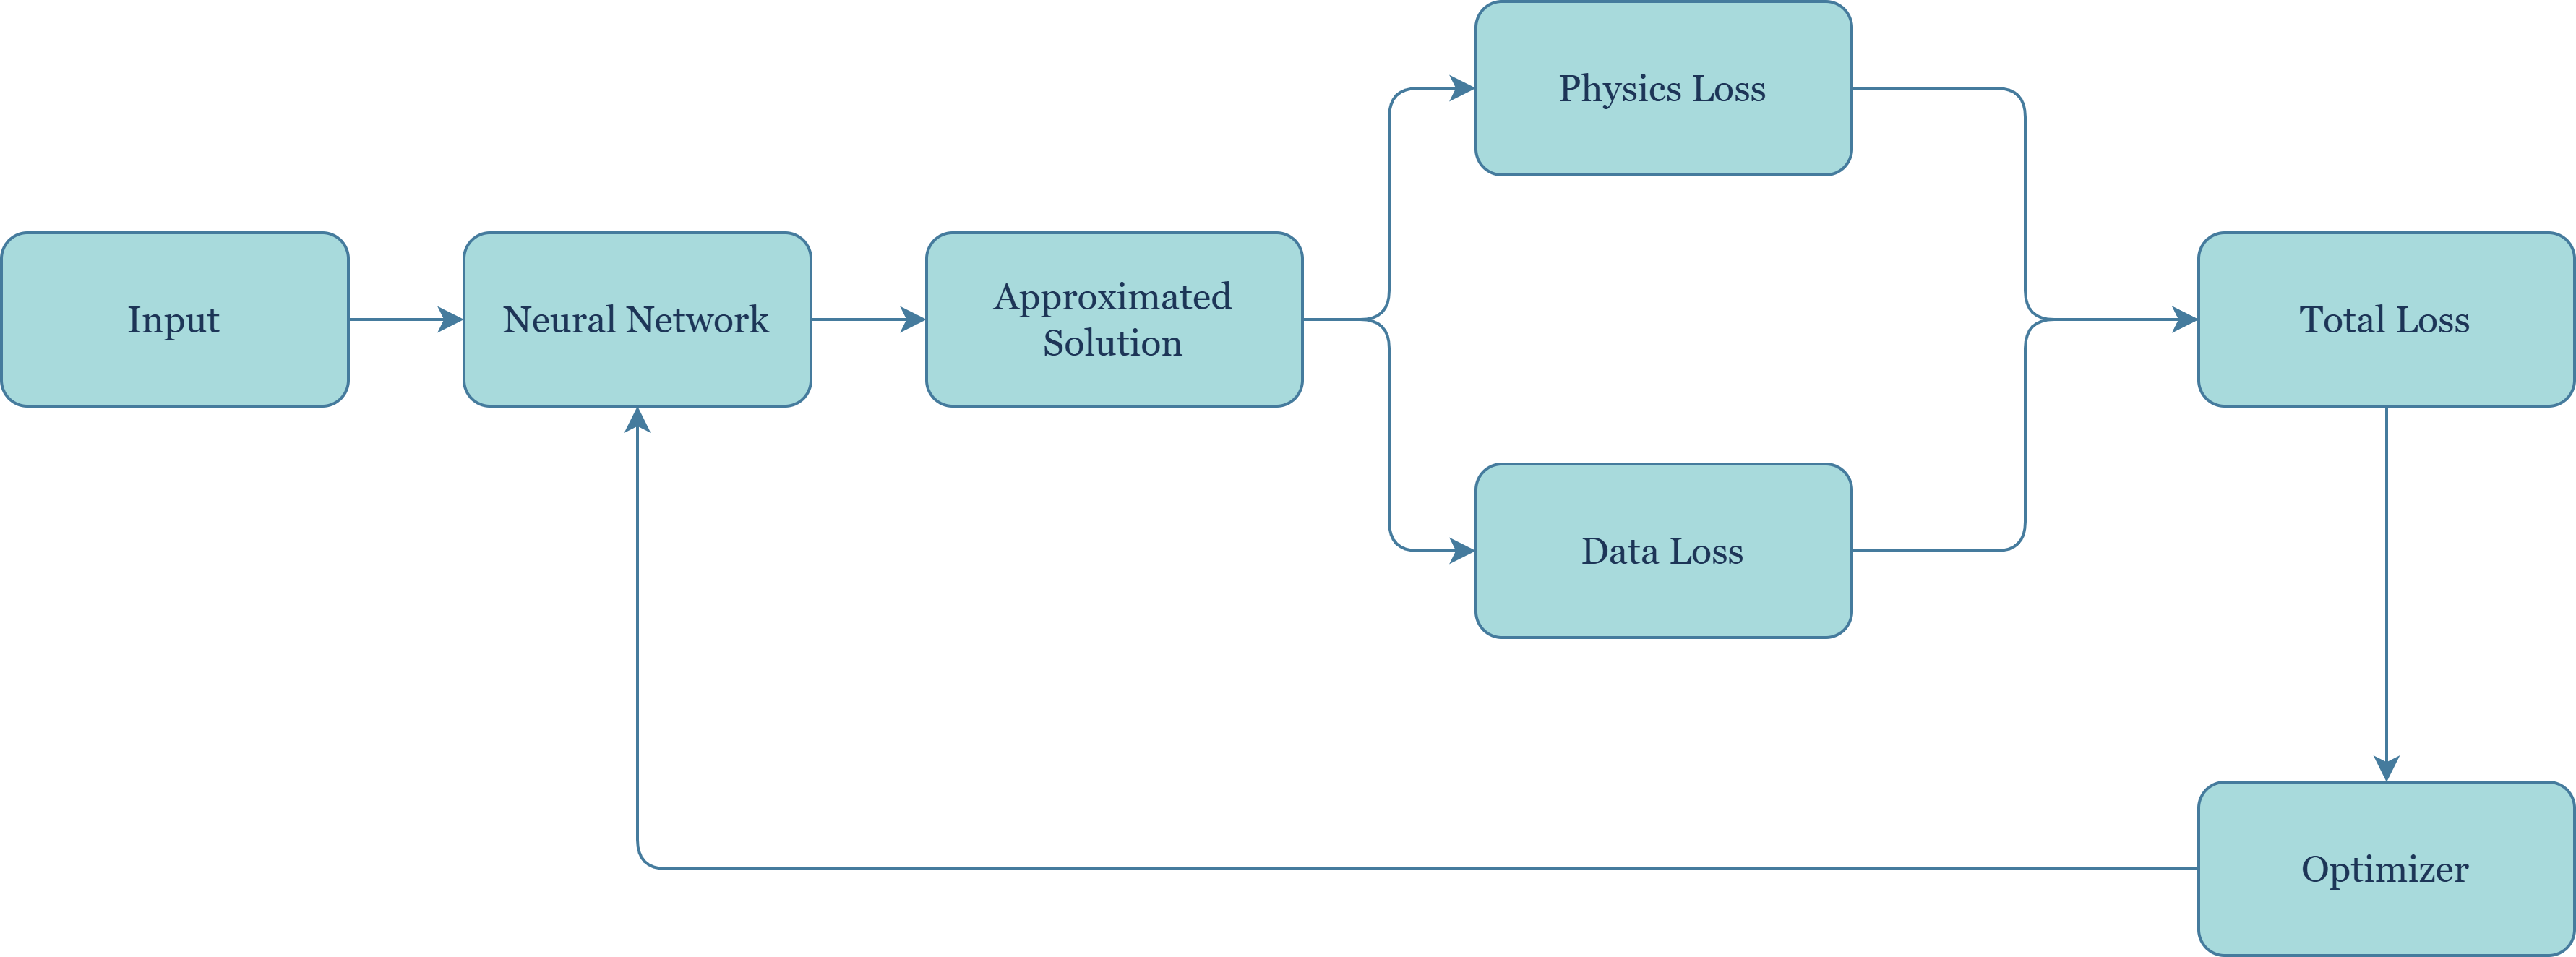
\includegraphics[width=1\textwidth]{images/pinn_framework.png}
	\caption{PINN Framework} 
	\label{fig:pinns}
\end{figure}


\subsection{Implenetation}

The architecture of a Physics-Informed Neural Network is typically implemented based on a 
fully connected feed-forward neural network, though in many cases they try many other architecture for NN. 
In this structure, the input layer receives the independent variables of 
the problem. For a time-dependent one-dimensional PDE, these inputs are 
usually the spatial coordinate $(x)$ and the time variable $(t)$. 
Therefore, each input point can be shown as $(x,t)$. The role of the 
neural network is mapping this input point to the corresponding approximation of the unknown solution. 
In other words, the network represents the function

\begin{equation}
	u_\theta(x,t) \approx u(x,t)
\end{equation}
where $(\theta)$ denotes all trainable parameters of the neural network, including weights and biases[lulu]

In the traditional neural network, the output of the architecture is checked only with available data. However, the output from the architecture in a PINN is
further taken to the physics-based part of the algorithm. 
This means that after the network predicts $u_\theta(x,t)$, automatic differentiation is applied to 
compute the derivatives required in the PDE, such as


\begin{equation}
	\frac{\partial u_\theta}{\partial t},
	\frac{\partial u_\theta}{\partial x},
	\frac{\partial^2 u_\theta}{\partial x^2}.
\end{equation}

\cite{Raissi2019}



To evaluate how well the governing equation is satisfied, 
PINNs introduce a set of collocation points inside the computational domain. 
These points are sampled throughout the domain and are not necessarily 
associated with any observed data. Let the collocation points be denoted by
${(x_f^i,t_f^i)}_{i=1}^{N_f}$

where $(N_f)$ represents the number of collocation points. 
At each of these points, the residual $(f_\theta(x,t))$ is evaluated. If the residual is large at a particular location, it indicates that the neural network 
prediction violates the governing 
equation at that point. Consequently, the network parameters are 
adjusted to reduce this error. One important advantage of this approach is 
that PINNs are mesh-free methods and therefore do not require the computational mesh used by traditional 
numerical techniques such as the Finite Element Method or Finite Difference Method. \cite{Raissi2019,Cuomo2022}


The learning process of a PINN is controlled through a loss function that combines 
information from both the available data and the governing physics. 
In the most general case, the total loss function consists of four components:
$$
\mathcal{L_{\textsl{data}}}
+
\mathcal{L_{\textsl{physics}}}
+
\mathcal{L_{\textsl{boundary}}}
+
\mathcal{L_{\textsl{initial}}}
$$

The data loss measures the difference between the neural network 
predictions and the available observations. The physics loss 
evaluates how well the governing differential equation is 
satisfied at the collocation points. The boundary loss enforces 
the prescribed boundary conditions, while the initial loss 
ensures that the initial conditions are satisfied. Together, 
these terms guide the network toward a physically meaningful solution.[raissi2019]
More specifically, the physics loss is often defined as the mean squared value of 
the PDE residual evaluated at all collocation points:
\begin{equation}
	\frac{1}{N_f}
	\sum_{i=1}^{N_f}
	\left|
	f_\theta(x_f^i,t_f^i)
	\right|^2
\end{equation}


Minimizing this term forces the neural network to satisfy the 
governing equation throughout the computational domain. Similarly, 
if observational data are available, the data loss can be written as


\begin{equation}
	\frac{1}{N_u}
	\sum_{i=1}^{N_u}
	\left|
	u_\theta(x_u^i,t_u^i)-u^i
	\right|^2,
\end{equation}

where $(u^i)$ denotes the observed value of the solution at the point $((x_u^i,t_u^i))$. [raissi2019]


After the total loss function is constructed, an optimization algorithm such 
as Adam or L-BFGS is used to update the trainable parameters $(\theta)$. 
During each training iteration, the gradients of the loss function with 
respect to the network parameters are computed using backpropagation. 
The optimization process continues until the total loss reaches a sufficiently 
small value, indicating that the neural network simultaneously fits the available 
data and satisfies the governing physical laws. \cite{Lu2021}



\subsection{The Schrödinger Equation and Physics-Informed Neural Networks}

The Schrödinger equation is the fundamental equation of quantum mechanics and 
describes the evolution of a quantum system through its wave function. In its 
time-dependent form, the equation is written as

\begin{equation}
	i\hbar \frac{\partial \psi}{\partial t}
	=
	\hat{H}\psi,
\end{equation}

where $\psi(x,t)$ denotes the wave function, $\hbar$ is the reduced 
Planck constant, and $\hat{H}$ is the Hamiltonian operator. 
The solution of the Schrödinger equation contains complete 
information about the physical system and can be used to 
determine quantities such as probability distributions and energy levels.

The Schrödinger equation plays a central role in many 
scientific fields, including quantum mechanics, 
quantum chemistry, atomic physics, 
condensed matter physics, and quantum computing. 
Because analytical solutions are available only for a 
limited number of simple systems, numerical methods are 
often required to approximate its solutions.

In recent years, Physics-Informed Neural Networks (PINNs) 
have emerged as a promising alternative to traditional numerical 
approaches. By embedding the governing differential 
equation directly into the loss function, PINNs can learn 
solutions that satisfy both observational data and the 
underlying physical laws. This capability makes PINNs particularly
attractive for solving Schrödinger-type equations, where accurate 
approximations of wave functions are required. \cite{Wang2021}

\subsection{Problem Statement}

In this project, we consider the one-dimensional time-dependent 
Schrödinger equation with a harmonic potential

\begin{equation}
	i\frac{\partial \psi}{\partial t}
	=
	-\frac{1}{2}\frac{\partial^2 \psi}{\partial x^2}
	+
	\frac{1}{2}x^2\psi,
\end{equation}

where $\psi(x,t)$ denotes the complex-valued wave function. The term

\begin{equation}
	-\frac{1}{2}\frac{\partial^2 \psi}{\partial x^2}
\end{equation}

represents the kinetic energy contribution, while

\begin{equation}
	\frac{1}{2}x^2\psi
\end{equation}

corresponds to the harmonic oscillator potential. 
This equation is one of the most important models in 
quantum mechanics and is frequently used as a benchmark 
problem for numerical and machine learning methods.

To solve this problem using PINNs, the neural 
network receives the spatial coordinate 
$x$ and time $t$ as inputs and approximates 
the wave function $\psi(x,t)$. Automatic d
ifferentiation is then employed to compute 
the derivatives required by the governing equation, 
and the residual of the Schrödinger equation is 
incorporated into the loss function. The network 
parameters are optimized such that the predicted 
solution satisfies both the differential equation 
and the prescribed initial and boundary conditions.
\subsection{Initial and Boundary Conditions}
To obtain a unique solution of the Schrödinger equation, 
appropriate initial and boundary conditions must be specified.
In this work, the spatial domain is defined as

\begin{equation}
	x \in [-5,5]
\end{equation}


while the temporal domain is chosen as

\begin{equation}
	t \in [0,1]
\end{equation}
The initial condition is selected as a Gaussian wave packet,

\begin{equation}
	\psi(x,0)=e^{-x^2}
\end{equation}

which is a commonly used initial state in quantum mechanics 
due to its smoothness and localized nature. Since the wave 
function is represented in terms of its real and imaginary 
components,

\begin{equation}
	\psi(x,t)=u(x,t)+iv(x,t)
\end{equation}

the initial condition can be written as

\begin{equation}
	u(x,0)=e^{-x^2}
\end{equation}


\begin{equation}
	v(x,0)=0
\end{equation}

These conditions are enforced during training through the initial-condition 
loss term, which penalizes discrepancies between the 
neural network predictions and the prescribed initial values.

Furthermore, homogeneous Dirichlet boundary conditions are 
imposed at the boundaries of the spatial domain. 
Specifically,

\begin{equation}
	u(-5,t)=u(5,t)=0
\end{equation}

and

\begin{equation}
	v(-5,t)=v(5,t)=0
\end{equation}


These boundary conditions ensure that the wave function 
remains negligible at the edges of the computational domain, 
which is consistent with the localized nature of the 
Gaussian initial state.

Within the PINN framework, 
both the initial and boundary conditions are 
incorporated directly into the loss function. 
During training, the neural network is required not 
only to satisfy the governing Schrödinger equation but 
also to reproduce the prescribed initial and boundary 
conditions. This enables the network to learn a physically 
consistent approximation of the wave function throughout 
the spatio-temporal domain.


\subsection{PINN Formulation for the Schrödinger Equation}

To solve the time-dependent Schrödinger equation using Physics-Informed Neural Networks (PINNs), the complex-valued wave function is first decomposed into its real and imaginary components. Thus, the solution is represented as

\begin{equation}
	\psi(x,t)=u(x,t)+i\,v(x,t)
\end{equation}

where $u(x,t)$ and $v(x,t)$ denote the real and imaginary parts of the wave function, respectively.

In the PINN framework, a fully connected neural network is employed to approximate these two functions simultaneously. The inputs of the network are the spatial coordinate $x$ and the time variable $t$, while the outputs correspond to the approximations $u_\theta(x,t)$ and $v_\theta(x,t)$, where $\theta$ denotes the trainable parameters of the neural network.

The governing equation considered in this work is

\begin{equation}
	i\frac{\partial \psi}{\partial t}
	=
	-\frac{1}{2}\frac{\partial^2\psi}{\partial x^2}
	+
	\frac{1}{2}x^2\psi
	\label{eq:schrodinger}
\end{equation}

Substituting

\begin{equation}
	\psi=u+i\,v
\end{equation}

into the Schrödinger equation and separating the real and imaginary parts yields the coupled system

\begin{equation}
	u_t
	=
	-\frac{1}{2}v_{xx}
	+
	V(x)v
\end{equation}

\begin{equation}
	v_t
	=
	\frac{1}{2}u_{xx}
	-
	V(x)u
\end{equation}

where

\begin{equation}
	V(x)=\frac{1}{2}x^2
\end{equation}

is the harmonic potential.

Using automatic differentiation, the neural network computes the required derivatives $u_t$, $v_t$, $u_{xx}$, and $v_{xx}$. These derivatives are then used to construct the physics residuals

\begin{equation}
	f_u
	=
	u_t
	+
	\frac{1}{2}v_{xx}
	-
	V(x)v
\end{equation}

\begin{equation}
	f_v
	=
	v_t
	-
	\frac{1}{2}u_{xx}
	+
	V(x)u
\end{equation}

If the neural network exactly satisfies the Schrödinger equation, both residual functions vanish throughout the computational domain. Therefore, the objective of the PINN is to minimize these residuals while simultaneously satisfying the prescribed initial and boundary conditions.

To enforce the governing equation, a set of collocation points is sampled inside the spatio-temporal domain. At these points, the residuals $f_u$ and $f_v$ are evaluated and incorporated into the loss function. The resulting physics loss is given by

\begin{equation}
	\mathcal{L}_{\mathrm{PDE}}
	=
	\frac{1}{N_f}
	\sum_{i=1}^{N_f}
	\left(
	|f_u(x_i,t_i)|^2
	+
	|f_v(x_i,t_i)|^2
	\right)
\end{equation}

where $N_f$ denotes the number of collocation points.

The total loss function combines the physics loss with the losses associated with the initial conditions, boundary conditions, and available reference data. Therefore,

\begin{equation}
	\mathcal{L}
	=
	\lambda_{\mathrm{PDE}}\mathcal{L}_{\mathrm{PDE}}
	+
	\lambda_{\mathrm{IC}}\mathcal{L}_{\mathrm{IC}}
	+
	\lambda_{\mathrm{BC}}\mathcal{L}_{\mathrm{BC}}
	+
	\lambda_{\mathrm{Data}}\mathcal{L}_{\mathrm{Data}}
\end{equation}

where the coefficients $\lambda_{\mathrm{PDE}}$, $\lambda_{\mathrm{IC}}$, $\lambda_{\mathrm{BC}}$, and $\lambda_{\mathrm{Data}}$ control the contribution of each component during training.
\subsection{Experimetal Setup}

The Physics-Informed Neural Network used in this work is implemented as a fully connected feed-forward neural network. The input layer receives the spatial coordinate $x$ and the time variable $t$, while the output layer predicts the real and imaginary components of the wave function, $u_\theta(x,t)$ and $v_\theta(x,t)$. Consequently, the network has two input neurons and two output neurons.

To approximate the solution of the Schrödinger equation, the network consists of four hidden layers with 64 neurons in each layer. The hyperbolic tangent ($\tanh$) activation function is employed throughout the hidden layers. This activation function is commonly used in PINN applications because it is smooth, differentiable, and well suited for automatic differentiation. The network weights are initialized using the Glorot normal initialization method, which helps stabilize the training process and improves convergence.

During training, collocation points are sampled throughout the computational domain to enforce the governing differential equation. Additional points are selected on the initial surface and domain boundaries to impose the prescribed initial and boundary conditions. Furthermore, reference solution data are incorporated into the training process to improve the accuracy of the learned solution.

The training procedure begins with a forward pass through the neural network. Given an input pair $(x,t)$, the network predicts the corresponding values of $u_\theta(x,t)$ and $v_\theta(x,t)$. Automatic differentiation is then used to compute the required derivatives appearing in the Schrödinger equation, including $u_t$, $v_t$, $u_{xx}$, and $v_{xx}$. These derivatives are subsequently used to evaluate the PDE residuals and the corresponding loss terms.

The total loss function is obtained by combining the physics loss, initial-condition loss, boundary-condition loss, and data loss. Backpropagation is then employed to compute the gradients of the loss function with respect to the trainable parameters of the network. These gradients are used to iteratively update the weights and biases until the network converges to a satisfactory solution.

To optimize the network parameters, a two-stage training strategy is adopted. In the first stage, the Adam optimizer is used to rapidly explore the parameter space and obtain a reasonable approximation of the solution. Adam is particularly effective during the early stages of training because of its adaptive learning-rate mechanism. In the second stage, the L-BFGS optimizer is employed to further refine the solution and improve convergence. This hybrid optimization strategy is widely used in PINN applications because it combines the robustness of Adam with the high-accuracy convergence properties of L-BFGS.

After training is completed, the resulting neural network provides an approximation of the wave function throughout the entire spatio-temporal domain. The accuracy of the learned solution is assessed by comparing the PINN predictions with the reference numerical solution and evaluating the relative $L_2$ error.

\begin{figure}[h]
	\centering
	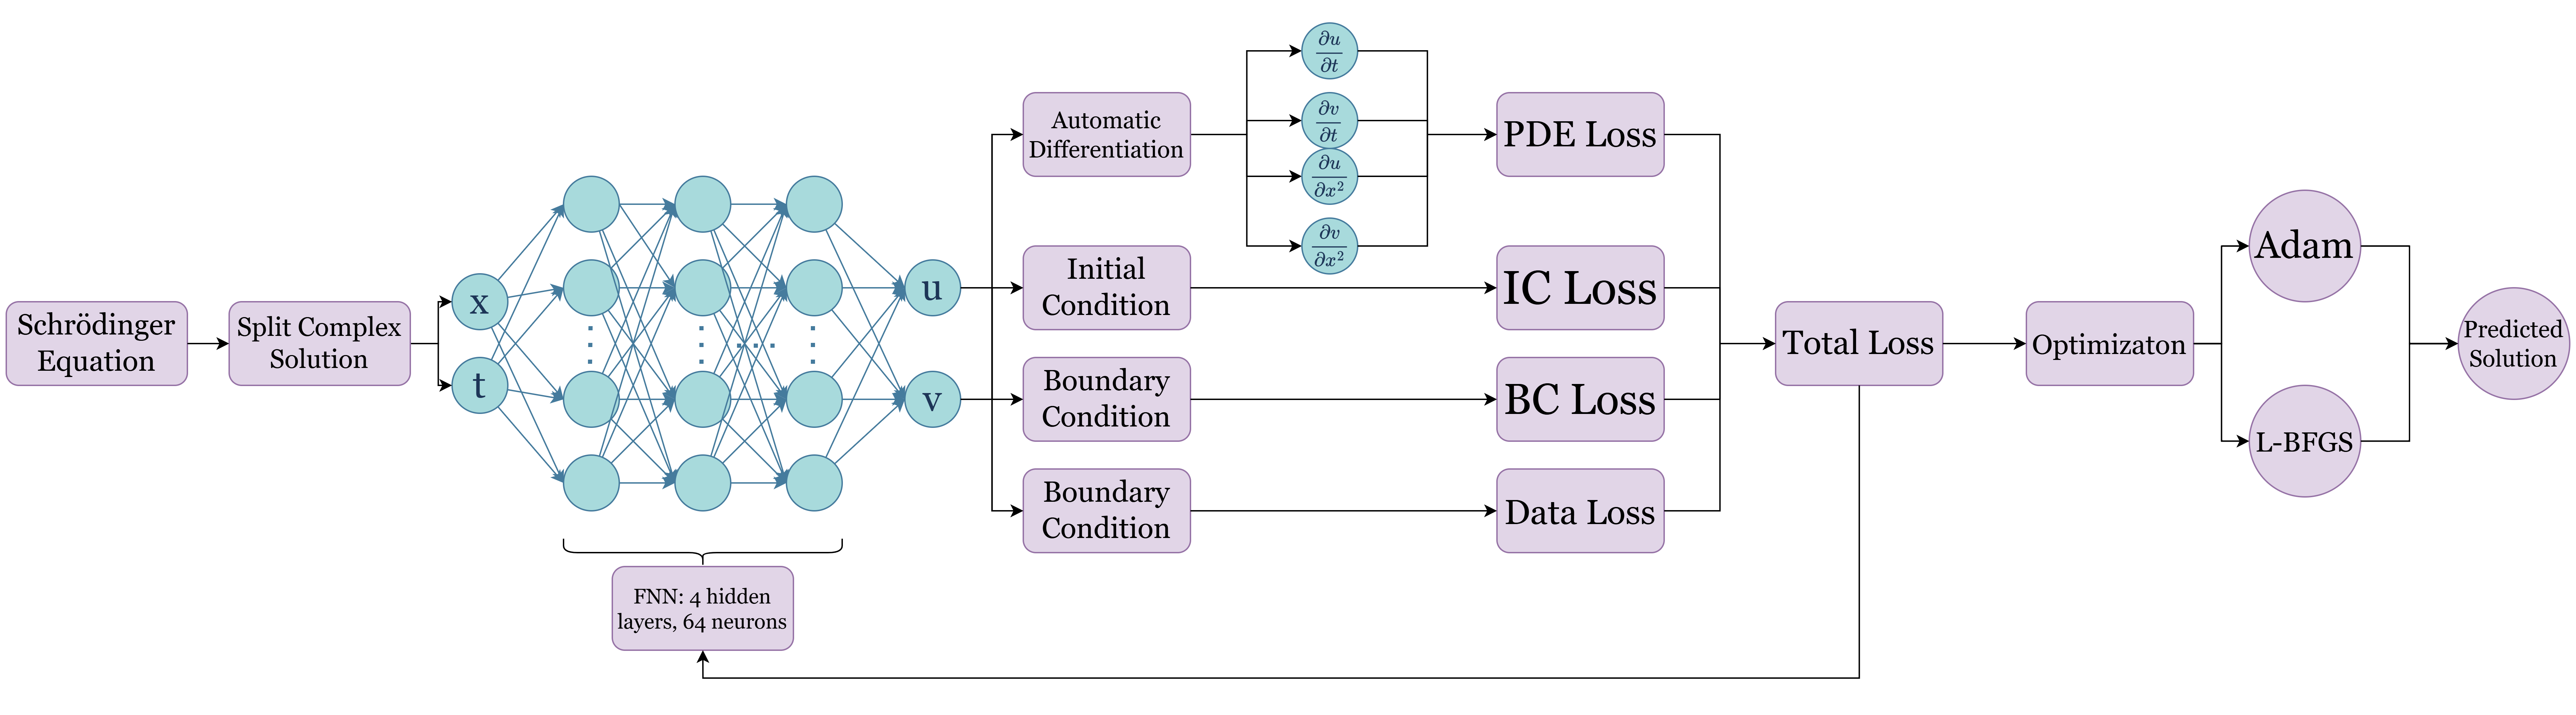
\includegraphics[width=1\textwidth]{images/SCH_diagram.png}
	\caption{Diagram of solving Schrodinger with PINN}
	\label{fig:sch1}
\end{figure}


\section{Results and Discussion}

This section presents the numerical results obtained using the proposed Physics-Informed Neural Network (PINN) for solving the one-dimensional time-dependent Schrödinger equation with a harmonic potential. The performance of the network is evaluated in terms of the training convergence and the predicted probability density of the wave function.

\subsection{Training Performance}

The network was trained using a two-stage optimization strategy. The Adam optimizer was first employed to obtain a suitable initial approximation of the solution, after which the L-BFGS optimizer was used to further refine the network parameters. This hybrid optimization strategy resulted in rapid convergence and a significant reduction in the overall loss.

After the Adam optimization stage, the total training loss decreased from approximately \(7.40 \times 10^{-3}\) to \(2.99 \times 10^{-6}\) following the L-BFGS optimization stage. The continuous reduction of the loss throughout training indicates that the neural network successfully learned the governing physics while satisfying the prescribed initial and boundary conditions. The final training and testing losses were nearly identical, suggesting that the network generalized well over the computational domain without noticeable overfitting.

\subsection{Probability Density Distribution}

Figure~\ref{fig:surface_density} illustrates the predicted probability density $|\psi(x,t)|^2$, over the entire spatio-temporal domain. The solution remains localized around the center of the spatial domain throughout the simulation. As time progresses, the probability density exhibits smooth temporal evolution while maintaining its overall symmetry. The obtained solution is continuous and free of numerical oscillations, demonstrating the capability of the PINN to approximate the solution over the entire computational domain.

\begin{figure}[h]
	\centering
	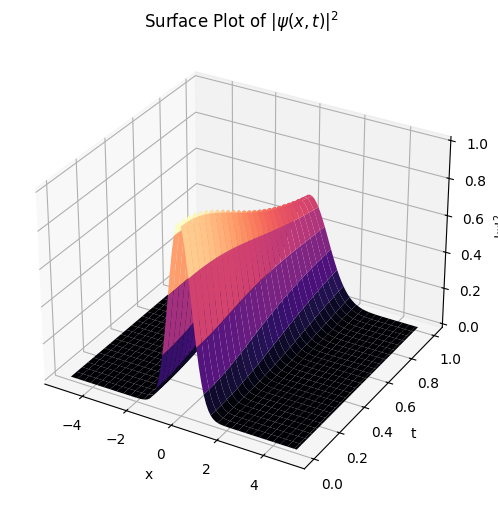
\includegraphics[width=7cm]{images/surface_density.png}
	\caption{Surface plot of the predicted probability density \(|\psi(x,t)|^2\).}
	\label{fig:surface_density}
\end{figure}

To further investigate the temporal evolution of the solution, the probability density was evaluated at several representative time instants, namely \(t=0\), \(0.25\), \(0.50\), \(0.75\), and \(1.00\). As shown in Figure~\ref{fig:selected_times}, the probability density evolves smoothly over time while preserving its symmetric profile about the center of the spatial domain.

\begin{figure}[h]
	\centering
	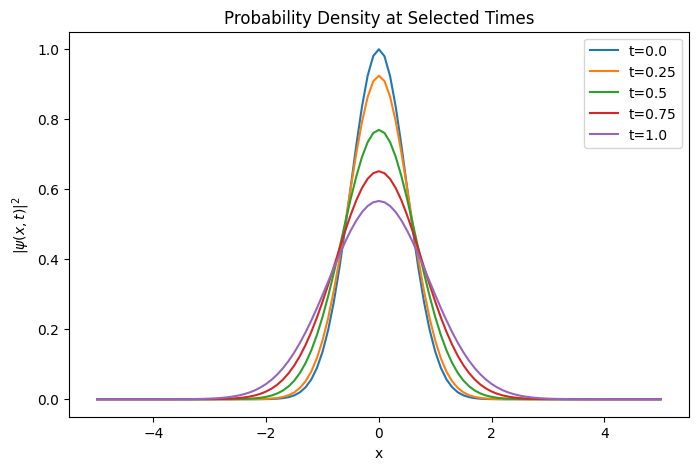
\includegraphics[width=7.5cm]{images/selected_times.png}
	\caption{Probability density \(|\psi(x,t)|^2\) at selected time instants.}
	\label{fig:selected_times}
\end{figure}

The curves remain smooth and symmetric about \(x=0\), indicating that the physical characteristics of the solution are preserved throughout the simulation. Moreover, the gradual transition between successive time levels demonstrates that the neural network accurately captures the temporal evolution of the wave function without introducing noticeable numerical artifacts.

\subsection{Discussion}

The obtained results demonstrate that the proposed PINN successfully approximates the solution of the one-dimensional time-dependent Schrödinger equation with high accuracy. The low final training loss, together with the smooth probability density distributions, indicates that the neural network satisfies both the governing differential equation and the prescribed initial and boundary conditions.

Furthermore, the predicted probability density exhibits physically consistent behavior throughout the computational domain. The absence of discontinuities and spurious oscillations suggests that automatic differentiation and the physics-informed loss function effectively guide the neural network toward a stable and physically meaningful solution.

Overall, these results confirm that Physics-Informed Neural Networks provide an effective framework for solving the time-dependent Schrödinger equation. By combining observational data with physics-based constraints, the proposed approach accurately reproduces the evolution of the quantum wave function while maintaining numerical stability throughout the simulation.

\begin{thebibliography}{99}
	\bibitem{Cuomo2022}
	S. Cuomo, V. Schiano di Cola, F. Giampaolo, G. Rozza, M. Raissi, and F. Piccialli,  
	“Scientific machine learning through physics-informed neural networks: Where we are and what’s next,”  
	\emph{Journal of Scientific Computing}, vol. 92, no. 3, Art. no. 88, 2022, doi: 10.1007/s10915-022-01939-z.
	
	\bibitem{Raissi2019}
	M. Raissi, P. Perdikaris, and G. E. Karniadakis,  
	“Physics-informed neural networks: A deep learning framework for solving forward and inverse problems involving nonlinear partial differential equations,”  
	\emph{Journal of Computational Physics}, vol. 378, pp. 686--707, 2019,  
	doi: 10.1016/j.jcp.2018.10.045.
	
	\bibitem{Lu2021}
	L. Lu, R. Pestourie, W. Yao, Z. Wang, F. Verdugo, and S. G. Johnson,  
	“Physics-informed neural networks with hard constraints for inverse design,”  
	\emph{SIAM Journal on Scientific Computing}, vol. 43, no. 6, pp. B1105--B1132, 2021,  
	doi: 10.1137/21M1397908.
	
	\bibitem{Wang2021}
	S. Wang, Y. Teng, and P. Perdikaris,  
	“Understanding and mitigating gradient flow pathologies in physics-informed neural networks,”  
	\emph{SIAM Journal on Scientific Computing}, vol. 43, no. 5, pp. A3055--A3081, 2021,  
	doi: 10.1137/20M1318043.

\end{thebibliography}
\end{document}
